%\documentclass[2p,11pt,number]{elsarticle}

\documentclass[preprint,12pt]{elsarticle}
\usepackage{amsmath,tikz,pifont,multicol,verbatim}

%\usepackage[margin=0.5in]{geometry}

\usepackage{hyperref,pgfplots}
\usepackage{subcaption}
\usepackage{cleveref}

\usepackage[export]{adjustbox}


\title{Families of Provably-stable Flux Reconstruction Schemes with Correction Functions Continuous in $m$ Derivatives}
\author[mrlm]{Manuel R. L\'opez Morales}
\author[ka]{Kartikey Asthana}
\address{Department of Aeronautics and Astronautics, Stanford University, Stanford, CA 94305, USA}
\date{\textsl{Aerospace Computing Laboratory}\\
March 24th, 2015}


% new commands

% % ---- graphics control
\newcommand{\graphWidth}{1.1}
\newcommand{\Ltrim}{3} % in cm
\newcommand{\Rtrim}{3} % in cm


%%----- from the internet
\newcommand*\circled[1]{\tikz[baseline=(char.base)]{
    \node[shape=circle,draw,inner sep=3pt] (char) {#1};}}
\newcommand*{\rom}[1]{\expandafter\@slowromancap\romannumeral #1@}
\providecommand{\e}[1]{\ensuremath{\times 10^{#1}}}


%%------ by author
\newcommand{\urd}{\hat{u}} % u reference discontinuous
\newcommand{\uud}{u} % u untransformed discontinuous
\newcommand{\frd}{{\hat{f}}} % f reference discontinuous
\newcommand{\fud}{f} % f untransformed discontinuous
\newcommand{\dd}[2]{{\frac{\partial #1}{\partial #2}}} % partial derivative
\newcommand{\dD}[2]{{#1}^{\l(#2\r)}} % partial derivative abbreviation
\newcommand{\ddxi}[1]{{\frac{\partial #1}{\partial \xi}}} % partial with respect to \xi
\newcommand{\ddxir}[2]{{\frac{\partial^{#2} {#1}}{\partial \xi^{#2}}}}
\newcommand{\DD}[2]{\frac{d #1}{d #2}} % total derivative
\newcommand{\dI}{{\delta I}} % delta I
\newcommand{\ioo}{{\int^1_{-1}}} % integral from -1 to 1
\newcommand{\IL}[1][i]{{I_{#1_{L,n}}}}
\newcommand{\IR}[1][i]{{I_{#1_{R,n}}}}
\newcommand{\gL}[1][i]{{g_{L_#1}}}
\newcommand{\gR}[1][i]{{g_{R_#1}}}
\newcommand{\urdrR}[1][n]{{\hat{u}^{(r)} \big|_{R,#1}}}
\newcommand{\urdrL}[1][n]{{\hat{u}^{(r)} \big|_{L,#1}}}
\newcommand{\uudrR}[1][n]{{{u}^{(r)} \big|_{R,#1}}}
\newcommand{\uudrL}[1][n]{{{u}^{(r)} \big|_{L,#1}}}
\newcommand{\uudrx}[2]{{{u}^{(r)}_{#1}(x_{#2})}}
\newcommand{\urdrx}[2]{{\hat{u}^{(r)}_{#1}(x_{#2})}}
\newcommand{\aL}[1][n]{{a_{r_{L,#1}}}}
\newcommand{\aR}[1][n]{{a_{r_{R,#1}}}}
\newcommand{\bOmega}{{\boldsymbol{\Omega}}}
\newcommand{\hu}{{\hat{u}}}
\newcommand{\hf}{{\hat{f}}}

\renewcommand{\th}{{^{\text{th}}}}
\renewcommand{\l}{\left}
\renewcommand{\r}{\right}
%\renewcommand{\thepage}{Version 3 -- Page \arabic{page} }



\begin{document}

% !TEX root = ./main.tex

\begin{abstract}
The goal of this paper is to present a verification and validation study of HiFiLES: a high-order LES solver developed in the Aerospace Computing Laboratory (ACL) at Stanford University. HiFiLES has been built on top of SD++ (Castonguay et al.) and achieves high-order spatial discretizations with the Energy-Stable Flux Reconstruction (ESFR) scheme on unstructured grids in two and three dimensions. The high parallelizability of this scheme motivates the optimization of the solver's ability to run in a multi-GPU (Graphical Processing Unit) environment.
We intend for this paper to be the main reference for HiFiLES and serve (with the previous SD++ papers) as a reference for researchers that would like to develop or implement high-order numerical schemes based on an Energy-Stable Flux Reconstruction (ESFR) approach.
\end{abstract}

\maketitle

\section{Introduction}
The \gls{fr} approach to high-order methods provides a unifying framework to analyze and implement a large set of high-order schemes, including the nodal \gls{dg} and \gls{sd} methods. The unification occurs through the formulation of flux correction functions. The main appeal of \gls{fr} is its differential formulation, which is ideal for highly-parallel computational architectures. \gls{esfr} provides the added benefit of guaranteeing linear stability while having variable dispersion and dissipation properties parameterized by a single constant. Asthana~\cite{asthana2014high} found optimal values for such constant and found that the \gls{fr} scheme could be optimized further if the scheme's formulation were not constrained by this parameter.

With the intention of providing a framework whereby more parameters are introduced while linear stability is guaranteed, we formulate the $C^m$ Flux Reconstruction (CMFR) set of families of schemes. The main difference between \gls{esfr} and \gls{cmfr} is that the flux correction functions in \gls{cmfr} are forced to be continuous among elements in an arbitrary number of derivatives, while \gls{esfr} requires $C^0$ and $C^{p+1}$ continuity only --where $p$ is the degree of the polynomial used to discretize the solution.

In this article we present the proof of linear stability of the \gls{cmfr} set of families of schemes, the derivation of C1FR --a \gls{fr} scheme with $C^1$ correction functions--, and promising results for energy preservation of underresolved wavenumbers with C1FR.

\section{The $C^m$ Flux Reconstruction Approach}

\subsection{Preliminaries: the general advection equation}
Suppose we would like to solve the one-dimensional conservation law
\begin{equation}
\label{eq:advec}
\dd{u}{t} + \dd{f}{x} = 0 
\end{equation}
in the domain $\bOmega$. $x$ is the spatial coordinate, $t$ is time, $u = u(x,t)$ is the conserved scalar quantity (or solution), and $f=f(u)$ is the flux. 

To discretize the equation, let us partition $\bOmega$ into $N$ non-overlapping elements $\bOmega_n = \{x | x_n < x < x_{n+1}\}$ and approximate both the solution $u$  and flux $f$ within each $\bOmega_n$ with polynomials. In each element, solution points are the locations where the solution values are stored and advanced; flux points in each element serve the same purpose for the flux values. In the Flux Reconstruction family of schemes, the solution and flux points are collocated in order to not have to compute additional flux interpolations.

As is customary, let us map the approximated solution and flux from the physical domain $\bOmega_n$ in $x$-coordinates to the reference domain $\hat{\Omega}=\{\xi | -1 < \xi < 1\}$ in $\xi$-coordinates. We can then write the approximations in the following form
\begin{align}
 \urd &= \sum^{P+1}_{p=1} \urd_p l_p(\xi) \\ 
 \frd &= \sum^{P+1}_{p=1} \frd(\urd_p)l_p(\xi)
\end{align}
where $P$ is the polynomial order used to represent the solution, $l_p$ is the Lagrange polynomial that equals $1$ at the solution/flux point $p$ and $0$ at the others, and $\urd_p$ is the solution value at the point $p$. Note that both $u$ and $f$ are potentially discontinuous across elements. 
The circumflex $\wedge$ means that the polynomial or entity below it is written or defined in reference domain coordinates.

Understanding that $J_n = \ddxi{x}\big|_n$,
we can rewrite Eqn.~\eqref{eq:advec} the reference domain coordinates
\begin{equation}
 \dd{\urd}{t} + \frac{1}{J_n}\ddxi{\frd} = 0 
\end{equation}

Let us clearly show the values of the desired $m^{\text{th}}$ order derivatives at the left interfaces of the $n^{\text{th}}$ element in
both the physical and reference domains.
\begin{align}
f\big|^{I}_{L,n} &= \frd\big|^{I}_{L,n} \\
\dd{f}{x} \bigg|_{L,n}^I &= \frac{1}{J_n} \ddxi{\frd}  \bigg|_{L,n}^I\\
\dd{^m f}{x^m} \bigg|_{L,n}^I &= \frac{1}{J_n^m} \dd{^m \frd}{\xi^m}  \bigg|_{L,n}^I
\end{align}

Here the symbol $|^{I}_{n,L}$ denotes that the quantity to its left is being evaluated at the \emph{left} ($L$) \emph{interface} ($I$) of element $n$, and $J_n$ represents the Jacobian of element $n$. Note that the desired interface values $\dd{^m \frd}{\xi^m}  \big|_{L,n}^I$ and $\dd{^m \frd}{\xi^m}  \big|_{R,n}^I$ will be defined later on when proving linear stability of the scheme.

It is important to note that
\begin{equation}
\dd{^m f}{\xi^m}  \bigg|_{R,n}^I = \dd{^m f}{\xi^m}  \bigg|_{L,n+1}^I
\end{equation}

Eventually, we would like to add a polynomial to the flux in order to guarantee continuity of arbitrary derivatives across elements. To that end, let us define the following correction constants at the left interface of element $n$ --the correction constants at the right interface are defined in the same way by replacing $L$ with $R$--

\begin{equation} 
\begin{aligned}
 \text{for $c^0$ continuity:} \, \IL[0] &= 
f\big|^I_{L,n} - \fud\big|_{L,n}\\
&= \frd\big|^I_{L,n} - \frd\big|_{L,n}\\
 &\vdots\\
\text{for $c^m$ continuity:} \, \IL[m] &= %
\dd{^m f}{x^m} \bigg|^I_{L,n} - \dd{^m \fud}{x^m} \bigg|_{L,n}\\
&= \frac{1}{J_n^m}\l(\dd{^m \frd}{\xi^m} \bigg|^I_{L,n} - \dd{^m \frd}{\xi^m} \bigg|_{L,n}\r)
\end{aligned}
\label{eq:jump_def}
\end{equation}
These constants are the difference between the desired flux derivative and the derivative of the flux polynomial at the interface of interest.

We can now introduce the correction functions that will enforce flux derivative continuity across elements. To guarantee that we have full control over which derivatives will be continuous at both the left ($L$) and right ($R$) interfaces at each element, we set the following conditions on the correction functions $\gL(\xi)$ and $\gR(\xi)$ defined in
element $n$ as follows:
\begin{equation}
\label{eq:gconstraints}
\begin{split}
&\dd{^j \gL}{x^j}(-1) = \delta_{ij} \; ; \; \dd{^j \gL}{x^j}(1) =
0 \\
&\dd{^j \gR}{x^j}(-1) = 0 \; ; \; \dd{^j \gR}{x^j}(1) = \delta_{ij}
%\frac{1}{J^j_n}
\end{split}
\end{equation}
where $\delta_{ij}$ is the Kronecker delta. $i$ and $j$ belong to the set of derivatives in which we wish to have continuity. For example, if we desire flux continuity in the zeroth and third derivatives, $i,j \subset \{0,3\}$. Note that the correction function polynomials must be of order greater than or equal to $2s$, where $s$ is the number of derivative continuities desired, due to the existence of two constraints per correction function. In the previous example, $s=2$.

Putting all the definitions together, we can now define the corrected flux in element $n$ as
\begin{equation}
\label{eq:f_corrected}
 \frd^{c} = \frd + \sum^m_{i=0}\left\{ \IL \gL + \IR \gR
 \right\}
\end{equation}
where $m$ is the highest derivative in which continuity is desired. The superscript $c$ is used to make it explicit that the quantity over which it appears has been made continuous across element interfaces. In the example, $m=3$, $I_{1_{L,n}} = I_{1_{R,n}} = I_{2_{L,n}} = I_{2_{R,n}} = 0$.
The semi-discrete form of the update step in element $n$ is
\begin{equation}
\DD{\urd_p}{t} = -\frac{1}{J_n} \left[ \ddxi{\frd}(\xi_p) + \sum_{i=0}^m \left\{ \IL
\ddxi{\gL}(\xi_p) + \IR \ddxi{\gR}(\xi_p)\right\} \right]
\end{equation}
for $p = 1,\ldots,P+1$. Note that the correction functions are being sampled at the same points as the flux and solution, so the fact that we are using polynomials of high orders as correction functions does not add computational complexity to the update step.
In vector form,
\begin{equation}
\DD{\overrightarrow{\urd}}{t} = -\frac{1}{J_n} \left[ \overrightarrow{\ddxi{\frd}} + \sum_{i=0}^m
\left\{ \IL
\overrightarrow{\ddxi{{\gL}}} + \IR \overrightarrow{\ddxi{{\gR}}}\right\}
\right]
\end{equation}

Here we see more clearly that the scheme maintains the desired computational parallelizability of the Flux Reconstruction family of schemes, as the only element specific values are the scalars $J_n$, $\IR$ and $\IL$.

\subsection{CMFR schemes for the general advection-diffusion equation}
The extension of a \gls{fr} scheme for the advection equation to the advection-diffusion equation is straightforward. If we want to solve
\begin{equation}
\label{eq:adv_diff}
\dd{u}{t} + \dd{f}{x} + \frac{\partial ^2 h}{\partial x^2}= 0 
\end{equation}
where $f$ and $h$ are functions of $u$, we can introduce an auxiliary variable $q$ so the equation becomes
\begin{equation}
\begin{split}
\dd{u}{t} + \dd{q}{x} &= 0\\
q &= f + \dd{h}{x} 
\end{split}
\end{equation}
Note that in the linear case, $h = -\beta u$ and $f = a u$.


When solving any \gls{pde}, the \gls{cmfr} schemes correct all functions dependent on $u$ whose first derivatives need to be found. In this general advection-diffusion case, $q$ and $h$ need to be corrected following the form in Eqn. \eqref{eq:f_corrected}. The main difference between this and the advection equation \gls{cmfr} scheme is that in this case there are two corrections necessary and the interface values $\IL,\IR$ used to correct $q$ will be a function of $q = f + \dd{h}{x}$ and not just $f$. The correction functions found for Eqn. \eqref{eq:f_corrected} remain exactly the same.

\section{Linear stability of $C^m$ continuous flux reconstruction $(\frd = a\urd)$}

In this section we show that the \gls{cmfr} schemes are stable in the 1-D linear advection equation in the following Sobolev-type norm:
\begin{equation}\label{eq:norm}
\begin{split}
|| \uud ||^2_m &=\sum_{n=1}^{N}\int_{x_n}^{x_{n+1}} \l\{ \sum^m_{r=0}
\frac{c_r}{2} \l( \dd{^r \uud}{x^r} \r)^2 \r\} dx \\
&=\sum_{n=1}^{N}   \sum^m_{r=0}
c_r \l(  \frac{1}{J_n^{2r}}\r) \ioo \l\{ \frac{1}{2}\l(\ddxir{\urd}{r} \r)^2
\r\} J_n \cdot d\xi 
\end{split}
\end{equation}
where $c_r$ for $0 \le r \le m$ are arbitrary constants. %To ensure Eqn.~\eqref{eq:norm}
%is a norm, let $c_0=1$. 
It is possible to find ranges of values of each $c_r$ for which Eqn. \eqref{eq:norm} is a norm. As shown later in section \ref{sec:advDiff}, negative values of $c_r$ are possible given that $\uud$ is a polynomial. To establish stability, we need to show that
\begin{equation}
\label{eq:ddnorm}
\DD{}{t}||\uud||^2_m = \sum_{n=1}^{N}   \sum^m_{r=0}
c_r \l(  \frac{1}{J_n^{2r}}\r) \DD{}{t}\ioo \l\{ \frac{1}{2}\l(\ddxir{\urd}{r} \r)^2
\r\} J_n \cdot d\xi \le 0
\end{equation} 

To that end, consider the \gls{fr} scheme in element $n$ for linear advection:
\begin{equation}
\label{eq:scheme}
\DD{\urd}{t} = -\frac{1}{J_n} \left[ a\ddxi{\urd} + \sum_{i=0}^m
\left\{ \IL
\ddxi{\gL} + \IR \ddxi{\gR}\right\} \right]
\end{equation}

To express Eqn. \eqref{eq:norm} in known terms, differentiate Eqn.
\eqref{eq:scheme} $r$ times, where $0\le r\le m$, with respect to $\xi$;
multiply by $\ddxir{\urd}{r}$; and integrate from $-1$ to $1$ to obtain
\begin{equation}
\label{eq:normterm1}
 \DD{}{t}\ioo \l\{ \frac{1}{2}\l( \ddxir{\urd}{r} \r)^2  \r\} d\xi = -\frac{1}{J_n}
\l[\text{\ding{172}}+\text{\ding{173}}+\text{\ding{174}} \r]
\end{equation}
where
\begin{align}
\label{eq:exp1}
 \text{\ding{172}}&= a \ioo \frac{1}{2} \ddxi{}\l( \ddxir{\urd}{r}\r)^2 d\xi=\frac{a}{2}\l[ 
\l( \ddxir{\urd}{r}\r)^2\bigg|_{R,n} - \l( \ddxir{\urd}{r}\r)^2\bigg|_{L,n} \r]\\
\label{eq:normterm2}
\text{\ding{173}}&= \sum^m_{i=0} \IL \ioo \ddxir{\urd}{r}\cdot \ddxir{\gL}{r+1} d\xi\\
\text{\ding{174}}&= \sum^m_{i=0} \IR \ioo \ddxir{\urd}{r}\cdot \ddxir{\gR}{r+1} d\xi
\end{align}


It is possible to simplify Eqn. \eqref{eq:normterm2} further.
% \begin{equation}
%  \text{\ding{173}}= \sum^m_{i=0} \IL \ioo \ddxir{\urd}{r}\cdot \ddxir{\gL}{r+1}
% d\xi\\
% \end{equation}
Integrating by parts,
\begin{align}
 \text{\ding{173}}&=\sum^m_{i=0} \IL \l\{ \ioo \l( \ddxi{} \l[ \ddxir{\urd}{r}
\ddxir{\gL}{r} \r]
-\ddxir{\gL}{r} \ddxir{\urd}{r+1} \r) d\xi \r\}\\
\text{\ding{173}}&= \sum^m_{i=0} \IL \l[\ddxir{\urd}{r} \ddxir{\gL}{r}\r]^1_{-1}
- \sum^m_{i=0} \IL \ioo
\ddxir{\gL}{r} \ddxir{\urd}{r+1} d\xi
\end{align}
By using the boundary conditions on $\gL$ given in Eqn.
\eqref{eq:gconstraints},
\begin{equation}
\label{eq:exp2}
\text{\ding{173}}=-\IL[r] J_n^r \ddxir{\urd}{r}\bigg|_{L,n} - \sum^m_{i=0} \IL \ioo
\ddxir{\gL}{r} \ddxir{\urd}{r+1} d\xi 
\end{equation}
Proceeding similarly with term \ding{174}
\begin{equation}
\label{eq:exp3}
\text{\ding{174}}=\IR[r] J_n^r\ddxir{\urd}{r}\bigg|_{R,n} - \sum^m_{i=0} \IR \ioo
\ddxir{\gR}{r}
\ddxir{\urd}{r+1} d\xi
\end{equation}

Note the difference in signs between \ding{173} and \ding{174}.

By replacing the expression from Eqn.~\eqref{eq:normterm1} into Eqn.~\eqref{eq:ddnorm}, we
obtain
\begin{equation}
\begin{split}
\label{eq:newnorm}
 \DD{}{t}&||\uud||^2_m = \sum_{n=1}^{N}\bigg\{   
\sum^m_{r=0}c_r \l(  -\frac{1}{J_n^{2r}}\r)  \frac{a}{2}\l[\l(
\ddxir{\urd}{r}\r)^2\bigg|_{R,n} - \l(\ddxir{\urd}{r}\r)^2\bigg|_{L,n} \r]  \\
&+ \sum^m_{r=0} c_r \l( - \frac{1}{J_n^{2r}}\r)  \l[ -\IL[r] J_n^r\ddxir{\urd}{r}
\bigg|_{L,n} - \sum^m_{i=0} \IL \ioo \ddxir{\gL}{r} \ddxir{\urd}{r+1} d\xi\r]\\
&+ \sum^m_{r=0} c_r \l( - \frac{1}{J_n^{2r}}\r)  \l[ \IR[r] J_n^r\ddxir{\urd}{r}
\bigg|_{R,n} -\sum^m_{i=0} \IR \ioo \ddxir{\gR}{r} \ddxir{\urd}{r+1} d\xi\r]\bigg\}
\end{split}
\end{equation}

%Notes: $g$ can be of any order as long as boundary constraints are satisfied. In other words, as will be seen later, $g$ must be at least of order $2(s+1)$ where $s$ is the number of types of flux continuities desired. If $g$ is $\mathcal{O}(p+s) ,s>1 \rightarrow$  cannot include $p\th$ order terms (simply) unless $c^p$ continuous. 

To de-clutter the notation, let us define $$\ddxir{*}{r} = \dD{*}{r} $$ and re-arrange Eqn.~\eqref{eq:newnorm} to obtain
\begin{equation}
\label{eq:timenorm}
 \DD{}{t}||\urd||^2_m = \text{\textcircled{a}} + \text{\textcircled{b}} + \text{\textcircled{c}}
\end{equation}
where
\begin{equation}
\begin{split}
 \label{eq:simpNormA}
 \text{\textcircled{a}} = -\sum_{n=1}^{N}  \bigg\{& 
 \sum^m_{r=0} c_r  \frac{a}{2} 
 \l[ \urd^{{(r)}^2} \big|_{R,n} - \urd^{{(r)}^2} \big|_{L,n} \r] 
 \l( \frac{1}{J_n^{2r}} \r) \\
 +& \sum^m_{r=0} -c_r \IL[r] J_n^r\urd^{(r)} \big|_{L,n} \l(
\frac{1}{J_n^{2r}}\r)\\
 +& \sum^m_{r=0} c_r \IR[r] J_n^r\urd^{(r)} \big|_{R,n} \l( \frac{1}{J_n^{2r}}\r)
 \bigg\} 
\end{split}
\end{equation}
\begin{equation}\label{eq:b_def}
 \text{\textcircled{b}} = \sum_{n=1}^{N} \l\{ 
 \sum^m_{r=0} c_r \sum^m_{i=0} \IL \ioo \dD{\gL}{r} \hat{u}^{{ (r+1)}} d\xi \l(
\frac{1}{J_n^{2r}}\r) \r\}
\end{equation}
\begin{equation}\label{eq:c_def}
 \text{\textcircled{c}} = \sum_{n=1}^{N}  \l\{ 
 \sum^m_{r=0} c_r \sum^m_{i=0} \IR \ioo \dD{\gR}{r} \hat{u}^{{ (r+1)}} d\xi \l(
\frac{1}{J_n^{2r}}\r) \r\}
\end{equation}


We show stability of \gls{cmfr} in the two following steps:
\begin{enumerate}
 \item We show that for a selection of interface values $\IL $ and $\IR $, 
 \begin{equation}\label{eq:a_le_0}
\text{\textcircled{a}} \le 0
 \end{equation}
 \item We explain how to find functions $\gL $ and $\gR $, for $i = 0,\ldots,m $ satisfying
conditions \eqref{eq:gconstraints} such that
\begin{equation}\label{eq:bc_equal_0}
\begin{split}
\text{\textcircled{b}}&=0\\
\text{\textcircled{c}}&=0
\end{split}
\end{equation}  
 for arbitrary
$c_r, r=1,\ldots,m$.
\end{enumerate}

By showing that expressions \eqref{eq:a_le_0} and \eqref{eq:bc_equal_0} hold, we conclude, from Eqn. \eqref{eq:timenorm} that
\begin{equation}
\DD{}{t}||\urd||_m \le 0
\end{equation}

\subsection{Part 1.}

In this part of the proof, we aim to show that the term \textcircled{a} in
Eqn.~\eqref{eq:timenorm} is non-positive.
\\
Rearranging and factoring terms in \textcircled{a}, Eqn. \eqref{eq:simpNormA} becomes
\begin{equation}
\begin{split}
\text{\textcircled{a}} =& -\sum_{n=1}^{N}  \bigg\{
 \sum^m_{r=0} c_r \l( \frac{1}{J_n^{2r}}\r)
 \bigg( \frac{a}{2} 
 \l[ \hat{u}^{{(r)}^2} \big|_{R,n} - \hat{u}^{{ (r)}^2} \big|_{L,n} \r]\\
 &- \IL[r] J_n^r\cdot \dD{\urd}{r} \big|_{L,n}
 +   \IR[r] J_n^r\cdot \dD{\urd}{r} \big|_{R,n}  \bigg)
 \bigg\}
 \end{split}
 \label{eq:aterm}
\end{equation}

Recall the definition of the correction constants $\IL[r] $ and
$\IR[r]$ in element $n$ from Eqn. \eqref{eq:jump_def},
\begin{equation}
\begin{split}
 \IL[r]J_n^r &= \dD{f}{r} \big|^I_{L,n} - {f}^{ (r)} \big|_{L,n}\\
 \IR[r]J_n^r &= \dD{f}{r} \big|^I_{R,n} - {f}^{ (r)} \big|_{R,n}
\end{split}
\end{equation}

In the case of linear advection, $\hat{f}^\delta = a\urd$, so the correction constants become
\begin{equation}
\label{eq:lincor}
\begin{split}
 \IL[r]J_n^r &= \dD{\hat{f}}{r} \big|^I_{L,n} - a\urdrL\\
 \IR[r]J_n^r &= \dD{\hat{f}}{r} \big|^I_{R,n} - a\urdrR
\end{split}
\end{equation}

Let us introduce the following generalized Roe flux at the interfaces, so
\begin{equation}
\label{eq:ifluxdef}
\begin{split}
\dD{\hat{f}}{r} \big|^I_{L,n} = \frac{1}{2}& \l[a\urdrL[n] + 
a\urdrR[n-1] \r] \\
&- \frac{1-{\alpha_r}}{2} \l|A_{r_{L,n}}\r| \l[\urdrL - \urdrR[n-1] \r]\\
\dD{\hat{f}}{r} \big|^I_{R,n} = \frac{1}{2}& \l[a\urdrL[n+1] + 
a\urdrR[n] \r]\\
&- \frac{1-{\alpha_r}}{2} \l|A_{r_{R,n}}\r| \l[\urdrL[n+1] - \urdrR[n] \r]
\end{split}
\end{equation}

Where $A_{r_{L,n}}$ and $A_{r_{R,n}}$ are the Jacobian matrices corresponding to the
$r^{\text{th}}$ derivative of the flux at the left ($L$) and right ($R$) interfaces of element $n$.
Equivalently,
\begin{equation}
\begin{split}
 A_{r_{L,n}} &= \l[ \frac{d \big( \hat{f}^{(r)} \big)}{d \big( \hat{u}^{(r)} \big)}
\r]_{L,n}\\
 A_{r_{R,n}} &= \l[ \frac{d \big( \hat{f}^{(r)} \big)}{d \big( \hat{u}^{(r)} \big)}
\r]_{R,n}
\end{split}
\end{equation}

Numerically, $A_{r_{L,n}}$ and $A_{r_{R,n}}$ can be evaluated for the linear advection equation as
\begin{equation}
\begin{split}
 A_{r_{L,n}} &= \frac{a \urdrL[n] - a \urdrR[n-1]}{\urdrL[n] - \urdrR[n-1]} = a\\%\aL\\
 A_{r_{R,n}} &= \frac{a \urdrL[n+1] - a \urdrR[n]}{\urdrL[n+1] - \urdrR[n]} = a%\aR = \aL[n+1]
\end{split}
\end{equation}

% Note that in the case of linear advection, $\aR = \aL = a$ for all $n$ and $r$. We leave the
% subscripts to later show that \textcircled{a} is non-negative even when the flux in non-linear.

Note that $A_{r_{L,n}} = A_{r_{R,n-1}}$ even for non-linear fluxes by construction.

Plugging these values of $A_{r_{L,n}}$ and $A_{r_{R,n}}$ into Eqn. \eqref{eq:ifluxdef}, and
substituting the updated interface flux values $\dD{\hat{f}}{r} \big|^I_{L,n}$ and $\dD{\hat{f}}{r}
\big|^I_{R,n}$ into the definition of the interface correction values in Eqn. \eqref{eq:lincor},
we obtain

\begin{equation}
\begin{split}
 \IL[r] J_n^r = \frac{1}{2} &\l\{a\urdrL[n] + 
a\urdrR[n-1] \r\}\\
 &- \frac{1-{\alpha_r}}{2} \l|a\r| \l\{\urdrL - \urdrR[n-1] \r\} - a\urdrL\\
 \IR[r] J_n^r = \frac{1}{2} &\l\{a\urdrL[n+1] + 
a\urdrR[n] \r\} \\
&- \frac{1-{\alpha_r}}{2} \l|a\r| \l\{\urdrL[n+1] - \urdrR[n] \r\} - a\urdrR
\end{split}
\end{equation}

Simplifying,
\begin{equation}
\label{eq:lincorUpdated}
\begin{split}
 \IL[r] J_n^r= \frac{a}{2}& \l\{-\urdrL[n] + \urdrR[n-1] \r\} \\
 &- \frac{1-{\alpha_r}}{2} \l|a\r| \l\{\urdrL
- \urdrR[n-1] \r\} \\
 \IR[r] J_n^r= \frac{a}{2}& \l\{\mbox{\;\;\:} \urdrL[n+1] - \urdrR[n] \r\} \\
 &- \frac{1-{\alpha_r}}{2}
\l|a\r|\l\{\urdrL[n+1] - \urdrR[n] \r\} 
\end{split}
\end{equation}


Using the updated values of $\IL[r]$ and $\IR[r]$ from Eqn. \eqref{eq:lincorUpdated},
Eqn. \eqref{eq:aterm} becomes
\begin{equation}
\begin{split}
 \text{\textcircled{a}} = -\sum_{n=1}^{N}  \bigg\{
 \sum^m_{r=0} & c_r \l( \frac{1}{J_n^{2r}}\r)
 \bigg( \frac{a}{2} 
 \l[ \hat{u}^{{ (r)}^2} \big|_{R,n} - \hat{u}^{{ (r)}^2} \big|_{L,n} \r] \\
 %
 &- \bigg[ \frac{a}{2} \l\{-\urdrL[n] + \urdrR[n-1] \r\} \\
 &\mbox{\;\;\;} - \frac{1-{\alpha_r}}{2} \l|a\r| \l\{\urdrL
- \urdrR[n-1] \r\} \bigg]  \cdot \urdrL\\
 &+  \bigg[ \frac{a}{2} \l\{\mbox{\;\;\:} \urdrL[n+1] - \urdrR[n] \r\} \\
 &\mbox{\;\;\;} - \frac{1-{\alpha_r}}{2} 
\l|a\r|
\l\{\urdrL[n+1] - \urdrR[n] \r\} \bigg]
 \cdot \urdrR 
\bigg)
 \bigg\} 
\end{split}
\end{equation}


Distributing the $\l(\frac{1}{J_n^{2r}}\r)$ term to convert the derivatives with respect to $\xi$
into derivatives with respect to $x$, and factoring out the $ \frac{a}{2}$ term,

\begin{equation}
\label{eq:termaphys}
\begin{split}
 \text{\textcircled{a}} = -\sum_{n=1}^{N}  \bigg\{
 \sum^m_{r=0} & c_r \frac{a}{2}
 \bigg(  
 \l[ {u}^{{ (r)}^2} \big|_{R,n} - {u}^{{ (r)}^2} \big|_{L,n} \r] \\
 %
 &- \bigg[ \l\{-\uudrL[n] + \uudrR[n-1] \r\} \\
 &\mbox{\;\;\;} - \frac{1-{\alpha_r}}{a} \l|a\r| \l\{\uudrL -
\uudrR[n-1] \r\} \bigg]
%
 \cdot \uudrL\\
 &+  \bigg[ \l\{\mbox{\;\;\:} \uudrL[n+1] - \uudrR[n] \r\} \\
 &\mbox{\;\;\;}- \frac{1-{\alpha_r}}{a} \l|a\r|
\l\{\uudrL[n+1] - \uudrR[n] \r\} \bigg]
 \cdot \uudrR 
\bigg)
 \bigg\} 
\end{split}
\end{equation}
%where the superscript $(r)$ now represents the $r^\text{th}$ derivative with respect to $x$.

Note that all terms in Eqn.~\eqref{eq:termaphys} are defined at element interfaces. More explicitly,
\begin{equation}
\label{eq:uudIdentities}
\begin{split}
\uudrL &= \uud_n(x_n) \\
\uudrR &= \uud_n(x_{n+1})
\end{split}
\end{equation}
where $\uud_n$ is the polynomial representing the solution in element $n$ and $x_n$ is the location
of the $n^\text{th}$ interface in physical coordinates.
Using the identities in Eqn.~\eqref{eq:uudIdentities}, Eqn.~\eqref{eq:termaphys} becomes
\begin{equation}
\label{eq:telSum0}
\begin{split}
 \text{\textcircled{a}} &= -\sum_{n=1}^{N}  \bigg\{
 \sum^m_{r=0} c_r \frac{a}{2}
 \bigg(  
 \l[ \l\{\uudrx{n}{n+1}\r\}^2  - \l\{\uudrx{n}{n}\r\}^2 \r] \\
 %
 &- \bigg[ \l\{-\uudrx{n}{n} + \uudrx{n-1}{n} \r\} \\
 &\mbox{\;\;\;}- \frac{1-{\alpha_r}}{a} \l|a\r|
\l\{\uudrx{n}{n} 
-
\uudrx{n-1}{n} \r\} \bigg]
%
 \cdot \uudrx{n}{n}\\
 &+  \bigg[ \l\{ \uudrx{n+1}{n+1} - \uudrx{n}{n+1} \r\} \\
 &\mbox{\;\;\;}- \frac{1-{\alpha_r}}{a} \l|a\r|
\l\{\uudrx{n+1}{n+1} - \uudrx{n}{n+1} \r\} \bigg]
 \cdot \uudrx{n}{n+1} 
\bigg)
 \bigg\} 
\end{split}
\end{equation}

Let us do the following substitutions to simplify algebraic manipulations
\begin{equation}
\label{eq:Bn}
\begin{split}
B_n = \sum^m_{r=0} c_r \frac{a}{2} \bigg( &\l[\uudrx{n-1}{n}\r]^2  \\
+ & \bigg[ \l\{\uudrx{n}{n} - \uudrx{n-1}{n} \r\} \\
&\mbox{\;\;\;}- \frac{1-{\alpha_r}}{a} \l|a\r| \l\{\uudrx{n}{n} 
- \uudrx{n-1}{n} \r\} \bigg] \cdot \uudrx{n-1}{n} \bigg)
\end{split}
\end{equation}

\begin{equation}
\label{eq:Dn}
\begin{split}
 D_n = \sum^m_{r=0} c_r \frac{a}{2} \bigg(- &\l[\uudrx{n}{n}\r]^2 \\
 - & \bigg[ \l\{-\uudrx{n}{n} + \uudrx{n-1}{n} \r\} \\
 &\mbox{\;\;\;}- \frac{1-{\alpha_r}}{a} \l|a\r|
\l\{\uudrx{n}{n} 
- \uudrx{n-1}{n} \r\} \bigg] \cdot \uudrx{n}{n} \bigg)
\end{split}
\end{equation}



We can then rewrite Eqn.~\eqref{eq:telSum0} as
\begin{equation}\label{eq:simple_summation}
  \text{\textcircled{a}} = -\sum_{n=1}^{N} \l\{ B_{n+1} + D_{n} \r\} 
\end{equation}

Let us manipulate \eqref{eq:simple_summation} to combine the two summations into one whose terms have the same unshifted index
\begin{equation}
\begin{split}
  \text{\textcircled{a}} &=  - \sum_{n=1}^{N} D_{n} -\sum_{n=1}^{N}  B_{n+1} \\
  \text{\textcircled{a}} &= - \sum_{n=1}^{N} D_{n} -\sum_{n=2}^{N+1}  B_{n}  \\
  \text{\textcircled{a}} &= - D_{1} - \sum_{n=2}^{N} D_{n}  - \sum_{n=2}^{N}  B_{n}  - B_{N+1} \\
  \text{\textcircled{a}} &= - D_{1} - \sum_{n=2}^{N} \l\{ D_{n}  +  B_{n} \r\}  - B_{N+1}
\end{split}
\end{equation}

Note that various terms in $B_n$ and $D_n$ cancel when summed (compare \eqref{eq:Bn} and \eqref{eq:Dn}). After doing such cancellations,
Eqn.~\eqref{eq:telSum0} becomes
\begin{equation}
 \text{\textcircled{a}} = -D_1 - \sum_{n=2}^{N} \sum^m_{r=0} c_r
\cdot \frac{1-\alpha_r}{2} |a| \l(\uudrx{n-1}{n} - \uudrx{n}{n} \r)^2 - B_{N+1} 
\end{equation}

The value of the solution and its derivatives at $x_1$ and $x_{N+1}$ are set by the desired boundary conditions. Both $D_1$ and $B_{N+1}$ depend exclusively on such pre-determined conditions:
% \begin{equation}
%  \uudrx{n}{n} = \uudrx{n-1}{n}
% \end{equation}
% As a result,
\begin{align}
 D_1 &= -\sum^m_{r=0} c_r\frac{a}{2} \l[ \uudrx{1}{1}\r]^2 \\
 B_{N+1} &= \sum^m_{r=0} c_r\frac{a}{2} \l[ \uudrx{N}{N+1}\r]^2
\end{align}

To not introduce/extract energy into/from the solution, let us set periodic boundary conditions in all derivatives,
\begin{equation}
 \uudrx{1}{1} = \uudrx{N}{N+1}
\end{equation}

Consequently, $D_1 + B_{N+1} = 0$, and Eqn.~\eqref{eq:telSum0} becomes simply
\begin{equation}
 \text{\textcircled{a}} = - \sum_{n=2}^{N} \sum^m_{r=0} c_r
\cdot \frac{1-\alpha_r}{2} |a| \l(\uudrx{n-1}{n} - \uudrx{n}{n} \r)^2
\end{equation}

Knowing that the following holds,
\begin{equation}
 \begin{split}
  c_r &\ge 0\\
  0 \le \alpha_r &\le 1\\
  \l(\uudrx{n-1}{n} - \uudrx{n}{n} \r)^2 &\ge 0  \mbox{ for } 2\le n \le N
 \end{split}
\end{equation}

we conclude that
\begin{equation}
 \text{\textcircled{a}} \le 0
\end{equation}


We have shown that the term \textcircled{a} in Eqn.~\eqref{eq:timenorm} is non-positive,
concluding this part of the proof.


\subsection{Part 2.}
We wish to find functions $\gL $ and $\gR $, for $i = 0,\ldots,m $,
which satisfy the boundary conditions in Eqn.~\eqref{eq:gconstraints} and the stability conditions of Eqn. \eqref{eq:bc_equal_0} (\textcircled{b}$=0$
and \textcircled{c}$=0$) for arbitrary
$c_r, r=1,\ldots,m$.

We start by finding $\gL$. Let us manipulate \textcircled{b} in Eqn. \eqref{eq:b_def} to find restrictions on $\gL$,

% done: 09/24/2014
\begin{equation}
\begin{split}\label{eq:b_cond}
 \text{\textcircled{b}} = \sum_{n=1}^{N} \l\{ 
 \sum^m_{r=0} \l[ c_r \l(
 \frac{1}{J_n^{2r}}\r) \sum^m_{i=0} \l( \IL \ioo \dD{\gL}{r} \hat{u}^{{ (r+1)}} d\xi \r) \r] \r\} &=0 \\
 = \sum_{n=1}^{N} \l\{ 
  \sum^m_{i=0} \l[ \IL \sum^m_{r=0} \l( c_r 
  \frac{1}{J_n^{2r}}  \ioo \dD{\gL}{r} \hat{u}^{{ (r+1)}} d\xi \r) \r] \r\} &=0
 \end{split}
\end{equation}

To satisfy Eqn. \eqref{eq:b_cond}, either
\begin{equation}
\label{eq:optionA}
\sum^m_{i=0}\l( \IL \ioo \dD{\gL}{r} \hat{u}^{{ (r+1)}}
d\xi \r) =0 
\end{equation}
or
\begin{equation}\label{eq:optionB}
\sum^m_{r=0} \l( c_r 
  \frac{1}{J_n^{2r}}  \ioo \dD{\gL}{r} \hat{u}^{{ (r+1)}} d\xi \r) =0
\end{equation}


We then have two options for finding $\gL$. Observing that the only term in the summand in \eqref{eq:optionB} that changes as the solution evolves is $\urd$ itself, we realize that a generic $\gL$ with special polynomial orthogonality properties would satisfy Eqn. \eqref{eq:b_cond}. As a result, we could pre-compute a non-changing $\gL$ to run a linearly stable scheme. On the other hand, the option given by \eqref{eq:optionA} obliges us to find
$\gL$ at every time-step because the scalar $\IL[i]$ changes with the solution. Therefore, we choose to find
$\gL$ using \eqref{eq:optionB}. %:
%\begin{equation}
%\label{eq:glcond}
% \sum^m_{r=0} c_r   \ioo \dD{\gL}{r} \hat{u}^{{\delta (r+1)}} d\xi \l(
%\frac{1}{J_n^{2r}}\r) =0 \text{ for each element $n$}
%\end{equation}


Rewriting $\urd$ as a sum of scaled Lagrange polynomials, condition \eqref{eq:optionB} becomes
\begin{equation}
 \label{eq:glcond1}  \sum^{P+1}_{p=1} \urd_p \sum^m_{r=0} \frac{c_r}{J^{2r}_n} \l(\ioo \dD{\gL}{r}
\dD{l_p}{r+1} d\xi \r) = 0
\end{equation}

This implies that
\begin{equation}\label{eq:glcond}
\sum^m_{r=0}\frac{c_r}{J^{2r}_n} \ioo \dD{\gL}{r} \dD{l_p}{r+1} d\xi = 0 
\end{equation}
for $p=1,\ldots, P+1$, (recall $P$ is the order of the polynomial used to represent $\urd$).
Let us expand the Lagrange polynomials $l_p$ and the correction functions $\gL$ into monomials,
\begin{equation}
\begin{split}
 l_p&=\sum^P_{j=0} \zeta_{pj} \xi^j\\
 \gL &= \sum^S_{k=0} \theta_{ik} \xi^k 
 \end{split}
\end{equation}
Note that $\zeta_{pj}$ are known, unchanging scalars while $\theta_{ik}$ are the unknowns we are trying to find. $S$ is the desired polynomial order of the correction function.

Eqn.~\eqref{eq:glcond} becomes
 \begin{equation*}
\sum^m_{r=0} \frac{c_r}{J^{2r}_n} \ioo 
\l( \sum^S_{k=r} \theta_{ik} \frac{k!}{(k-r)!} 
\xi^{k-r}  \r)
\l(
\sum^P_{j=r+1}\zeta_{pj}\frac{j!}{(j-r-1)!}  \xi^{j-r-1} \r)
d\xi =0
\end{equation*}

After some algebraic manipulation, we arrive at the conditions that each $\gL$ must satisfy so the \gls{cmfr} scheme maintains linear stability:
\begin{equation}
 \label{eq:gcond}
\sum^m_{r=0} \frac{c_r}{J^{2r}_n}  
\l[ \sum^S_{k=r} \theta_{ik} \frac{k!}{(k-r)!} 
\l(
\sum^P_{j=r+1}\zeta_{pj}\frac{j!}{(j-r-1)!}  \ioo \xi^{j+k-2r-1} d\xi\r)\r]
 =0
\end{equation}

Recall that $i$ in $\theta_{ik}$ indexes the correction function corresponding to each specific derivative in which continuity is desired. $p$ indexes each solution point in the reference domain.

With Eqn.~\eqref{eq:gcond} and the constraints given in Eqn.~\eqref{eq:gconstraints} we can
construct a system of equations to solve for $\gL$ in each element. More specifically, if we
would like to ensure $s$ different flux continuities between elements, the boundary constraints in
Eqn.~\eqref{eq:gconstraints} produce $2s$ equations, and the conditions in
Eqn.~\eqref{eq:gcond} produce $P$ equations (not necessarily all independent), where $P$ is the order of the solution
representation $\urd$. %Note, however, that if the flux continuity is desired in the $P+1^\text{th}$, or higher, derivative, the flux can be of order $2s+P-1+(-2)$ or higher, as the boundary conditions related to the $P+1^\text{th}$ derivative are satisfied automatically due to the fact that $\hat{u}^{\delta(P+1)}=0$ in every element.

We can recover the \gls{esfr} scheme by
ensuring continuity in the $0^\text{th}$ and $P+1^\text{th}$ derivatives. These two desired
flux continuities ($s=2$) force the flux to be of order, at least, $P+1$. This is the order of the correction functions suggested by Vincent~\cite{vincent2011new}. The \gls{esfr} scheme is one of the cases in which Eqn. \eqref{eq:glcond} produces $P-1$ independent equations instead of $P$. This can be seen by the fact that the $P+1^\text{th}$ and  $P+2^\text{th}$ derivatives of a Lagrange polynomial $l_p$ of order $P$ is zero.

Once we find $\gL$, we find $\gR$ automatically by setting 
\begin{equation}\label{eq:gr_gl_cond}
 \gR = (-1)^i\gL(-\xi)
\end{equation}
%in Eqn. \eqref{eq:c_def}.

\section{$C^{1}$ linearly stable flux reconstruction family of schemes}
In this section, we illustrate the process of creating a scheme that ensures $C^{1}$
flux continuity to solve the advection and advection-diffusion equation. This scheme is called C01FR, or \gls{c1fr}. We use this notation because it is possible to create a scheme whose reconstructed flux is continuous in the, say, zeroth and third derivatives without enforcing continuity in the first and second derivatives, and such scheme would have a $C^{0,3}$ flux and be called C03FR. When a scheme ensures continuity in the $0,\dots,M$ derivatives of the flux, we call it \gls{cmfr} to simplify the name, which could as well be C012...MFR.

\subsection{C1FR for the linear advection equation}
To create the scheme with $C^{1}$ flux, we only need to find correction functions $\gL$ that satisfy \eqref{eq:gcond} and boundary conditions \eqref{eq:gconstraints}.
Let $c_0$ and $c_1$ be non-zero in Eqn. \eqref{eq:gcond}. Expanding the summation over $r$, we have the following $P+1$ equations for each $i$

\begin{equation}
\begin{split}
c_0 &\l[ \sum^S_{k=0} \theta_{ik}\l( \sum^P_{j=1}\zeta_{pj}\cdot j\cdot \ioo  \xi^{j+k-1}d\xi \r) \r] \\
&+ 
\frac{c_1}{J^2_n} \l[ \sum^S_{k=1} k \theta_{ik} \l( \sum^P_{j=2}\zeta_{pj}\cdot j\cdot (j-1)\cdot \ioo  \xi^{j+k-3}d\xi \r) \r]
 = 0
 \end{split}
\end{equation}
for $p = 1,...,P+1$.

Rearranging terms we obtain
\begin{equation}
\begin{split}
\sum^P_{j=1} \zeta_{pj} &\bigg[ \sum^S_{k=0} \theta_{ik}\bigg( c_0\cdot  j \ioo  \xi^{j+k-1}d\xi  \\
&+ \frac{c_1}{J^2_n} k j\cdot (j-1)  \ioo  \xi^{j+k-3}d\xi \bigg) \bigg]
 = 0
 \end{split}
\end{equation}

and, therefore we have the following $P$ equations, where $j = 1,\dots,P$,
\begin{equation}
\label{eqn:system}
\sum^S_{k=0} \theta_{ik}\l( c_0\cdot  j \ioo  \xi^{j+k-1}d\xi  + \frac{c_1}{J^2_n} k j\cdot (j-1)  \ioo  \xi^{j+k-3}d\xi \r) = 0
\end{equation}

We can evaluate the integral terms understanding that for positive integer $q$
\begin{equation}
\ioo \xi^q d\xi = 
\l\{
\begin{array}{ll}
\frac{2}{q+1} & \mbox{, $q$ even}\\
0 & \mbox{, $q$ odd} 
\end{array}
\r.
\end{equation}

\begin{comment}
\begin{align}
 \ioo& \l\{ \gL\xi + \frac{c_1}{J_n^2} \ddxi{\gL}(j-1)\r\}\xi^{j-2} d \xi =0 \mbox{ for }
j=1,\ldots,m\\
 \implies &\sum^s_{k=0}\theta_{ik} \ioo \l\{ \xi^{k+1} + \frac{c_1}{J_n^2} k
\xi^{k-1}(j-1)\r\}\xi^{j-2}d\xi =0
\end{align}

We want to evaluate
\begin{equation}
 \ioo \l\{ \underbrace{\xi^{k+j-1}}_{\text{\ding{172}}} + \underbrace{\frac{c_1}{J_n^2} k (j-1)
\xi^{k+j-3}}_{\text{\ding{173}}} \r\} d\xi \mbox{ , } 0\le k\le s
\end{equation}

\ding{172}:

\begin{equation}
\ioo \xi^{k+j-1} d\xi = \frac{1}{k+j} \xi^{k+j} \bigg|^1_{-1} = \frac{1}{k+j} \l[ 1-(-1)^{k+j} \r]
\end{equation}

\ding{173}:
\begin{equation}
 \frac{1}{J_n^2}\ioo c_1 k (j-1) \xi^{k+j-3} d\xi = \frac{c_1}{J_n^2} k (j-1) \frac{1}{k+j-2} \l[
1-(-1)^{k+j-2} \r] \mbox{ for
} k+j\ne2
\end{equation}
If $k+j=2$, $j=2$ and $k=0$, so
\begin{equation}
 \ioo c_1 k (j-1) \xi^{k+j-3} d\xi = 0
\end{equation}

To find the coefficients of the monomials that describe $\gL$ and $\gR$, we want to write the
constraints in matrix form:
\begin{equation}
\label{eq:gcoeff}
 0=\sum^s_{k=0} \theta_{ik} \l\{  \frac{1}{k+j} \l[1-(-1)^{k+j}\r] + \frac{c_1}{J_n^2} k
\frac{j-1}{k+j-2} \l[
1-(-1)^{k+j-2} \r] \r\} \mbox{  for  } j=1,\ldots,p
\end{equation}

Note that for $j$ odd, Eqn.~\ref{eq:gcoeff} becomes
\begin{equation}
 0 = \sum^s_{\substack{k=0\\k \text{ even}}} \theta_{ik} \l\{ \frac{2}{k+j} +2 \frac{c_1}{J_n^2} k
\frac{j-1}{k+j-2}\r\}
\end{equation}

and for $j$ even, Eqn.~\ref{eq:gcoeff} becomes
\begin{equation}
 0 = \sum^s_{\substack{k=0\\k \text{ odd}}} \theta_k \l\{ \frac{2}{k+j} +2 \frac{c_1}{J_n^2} k
\frac{j-1}{k+j-2}\r\}
\end{equation}
\end{comment}
Recalling the constraints on $\gL$,
\begin{equation}
 g^{(j)}_{L_i}(-1) = \delta_{ij} J_n^j \; ; \;   g^{(j)}_{L_i}(+1) = 0
\end{equation}

we can obtain additional equations for each $\theta_{ik}$. Specifically, for $\gL[0]$,
\begin{equation}
\begin{split}
\sum^S_{k=0} \theta_{0k}(-1)^k = 1\hspace{0.7cm} \text{ \hspace{1cm} }
&\sum^S_{k=0}
\theta_{0k}(1)^k = 0\\
\sum^S_{k=1} k\theta_{0k}(-1)^{k-1} = 0 \text{ \hspace{1cm} } &\sum^S_{k=1}
k\theta_{0k}(1)^{k-1} = 0
\end{split}
\end{equation}
and for $\gL[1]$,

\begin{equation}
\begin{split}
\sum^S_{k=0} \theta_{1k}(-1)^k = 0\hspace{0.7cm} \text{ \hspace{1cm} }
&\sum^S_{k=0}
\theta_{1k}(1)^k = 0\\
\sum^S_{k=1} k\theta_{1k}(-1)^{k-1} = J_n \text{ \hspace{1cm}} & \sum^S_{k=1}
k\theta_{1k}(1)^{k-1} = 0
\end{split}
\end{equation}

From Eqn. \eqref{eq:gr_gl_cond}, we can find $\gR$ by setting
\begin{equation}
\gR = (-1)^i\sum_{k=0}^S \theta_{ik}(-\xi)^k = \sum_{k=0}^S \theta_{ik}(-1)^{i+k}\xi^k
\end{equation}

As a result, for each $\gL$ we have $P+4$ equations. By setting $S$, the order of the correction function, to be $P+3$, we have $P+4$ unknowns and can solve a $(P+4)\times(P+4)$ system of equations to have a one-parameter, linearly stable, $C^{1}$ flux, \gls{fr} scheme.

Letting the polynomial order $P$ be $3$, we obtain the correction functions seen in Fig. \ref{fig:c1_corfunc} for varying values of $c_1$. We let $c_0 = 1$ without loss of generality (as seen by the fact that in Eqn. \eqref{eqn:system} only the ratio $c_1/c_0$ modifies the correction functions). We note that the correction functions that ensure the flux is continuous in its first derivative, namely $\gL[1]$ and $\gR[1]$ are unaffected by changes in $c_1$. On the other hand, $\gL[0]$ and $\gR[0]$ change dramatically with changes in $c_1$. In section \ref{sec:num_cases} we will see how these variations affect dispersion and dissipation properties qualitatively.

In Fig. \ref{fig:c2_corfunc} we see the correction functions corresponding to the C012FR, or C2FR, scheme with $P=3$. It is interesting to note that changes in $c_1$ affect $\gL[0]$ and $\gR[0]$ only, changes in $c_2$ affect $\gL[1]$ and $\gR[1]$ only, and $\gL[2]$ and $\gR[2]$ are not affected by $c_1$ or $c_2$.

\begin{figure}[h]
\hspace{-1.25 cm}
\centering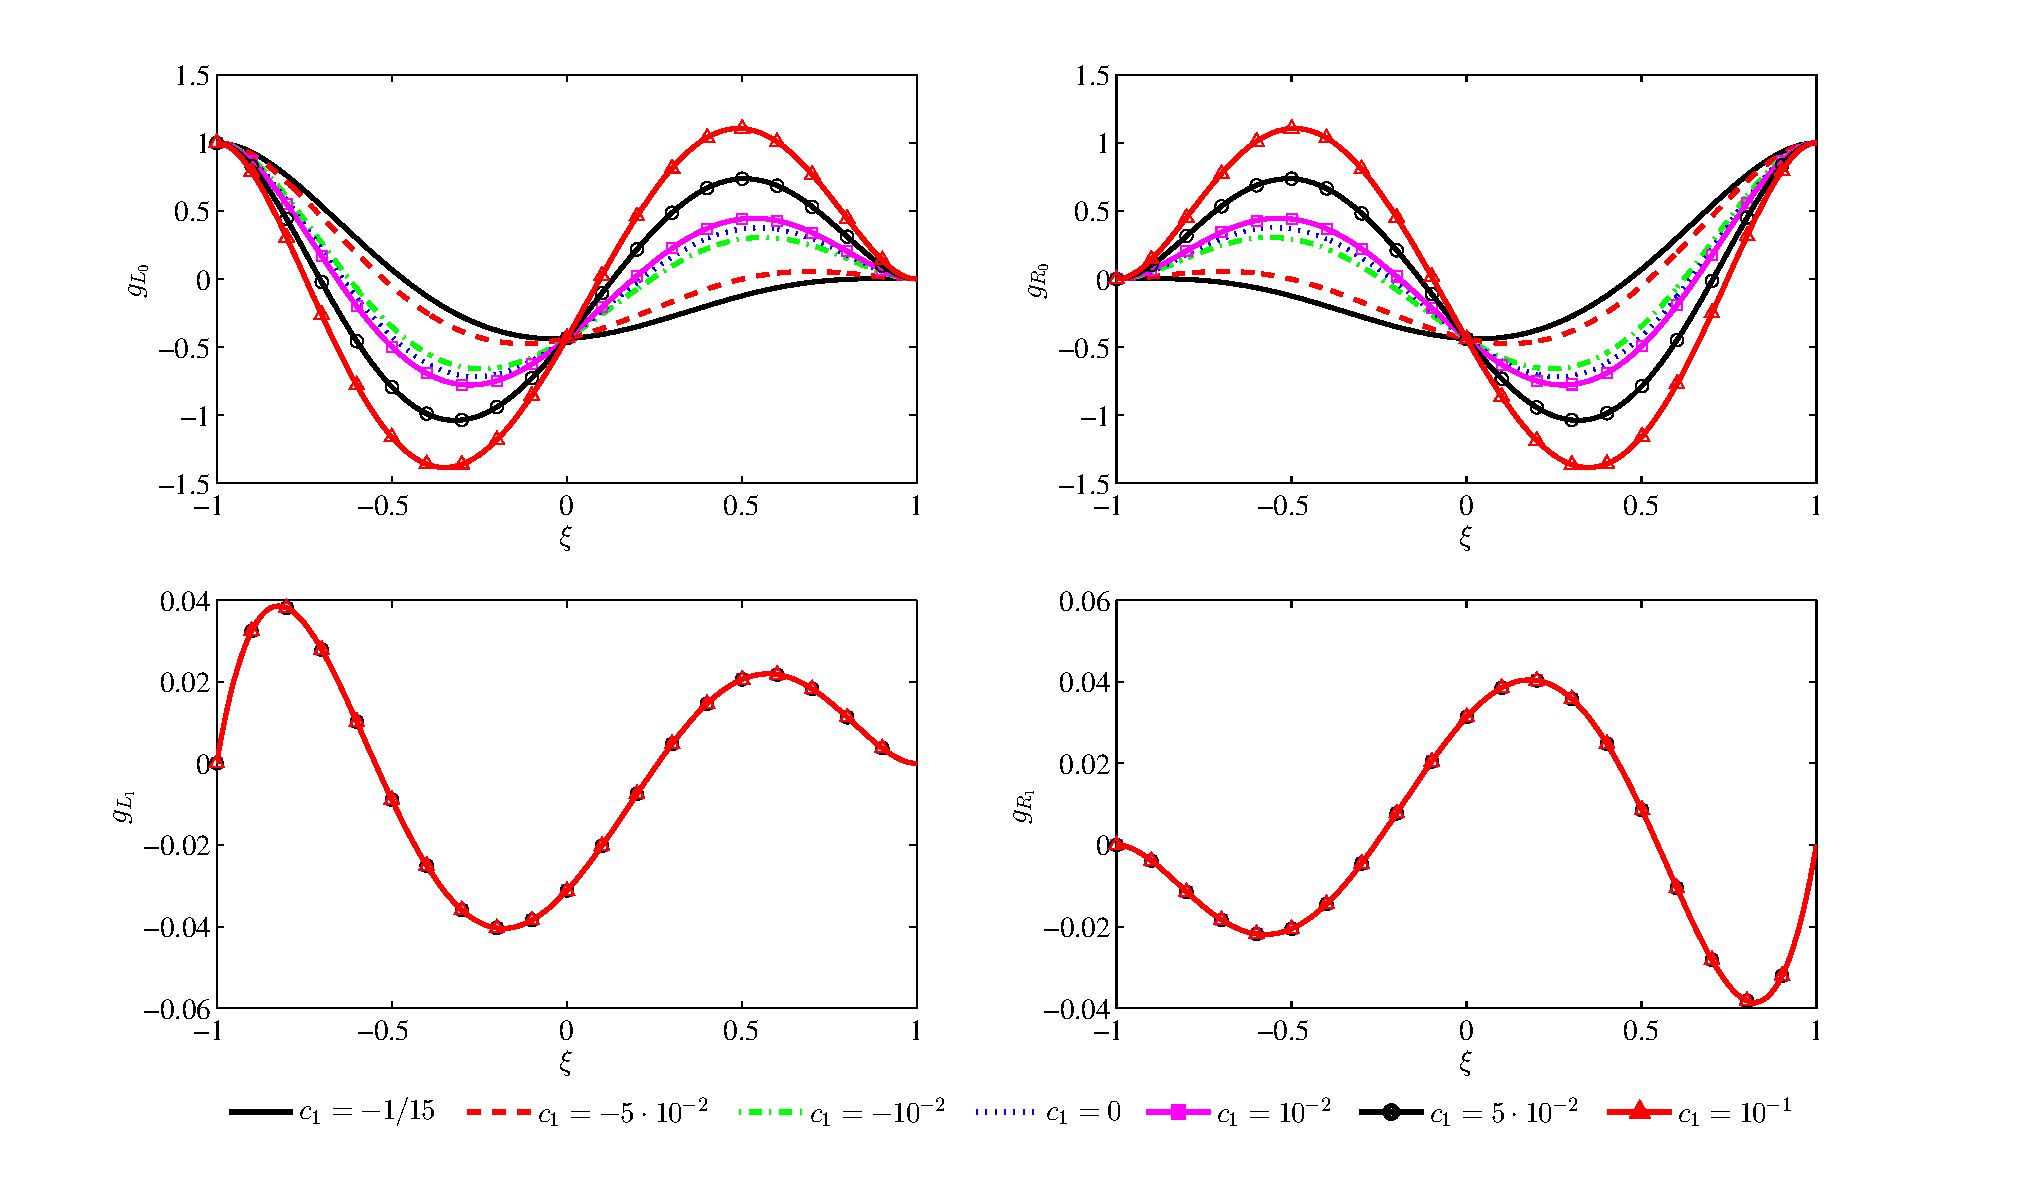
\includegraphics[width=\graphWidth\textwidth,trim=\Ltrim cm 0cm \Rtrim cm 0cm]{\cmfrdir/Figures/Correction_funcs/C1FR}
\caption{Left and right correction functions for the C1FR scheme with $P=3$, in which the zeroth and first derivatives of the corrected flux are continuous}
\label{fig:c1_corfunc}
\end{figure}

\begin{figure}[h]
\centering 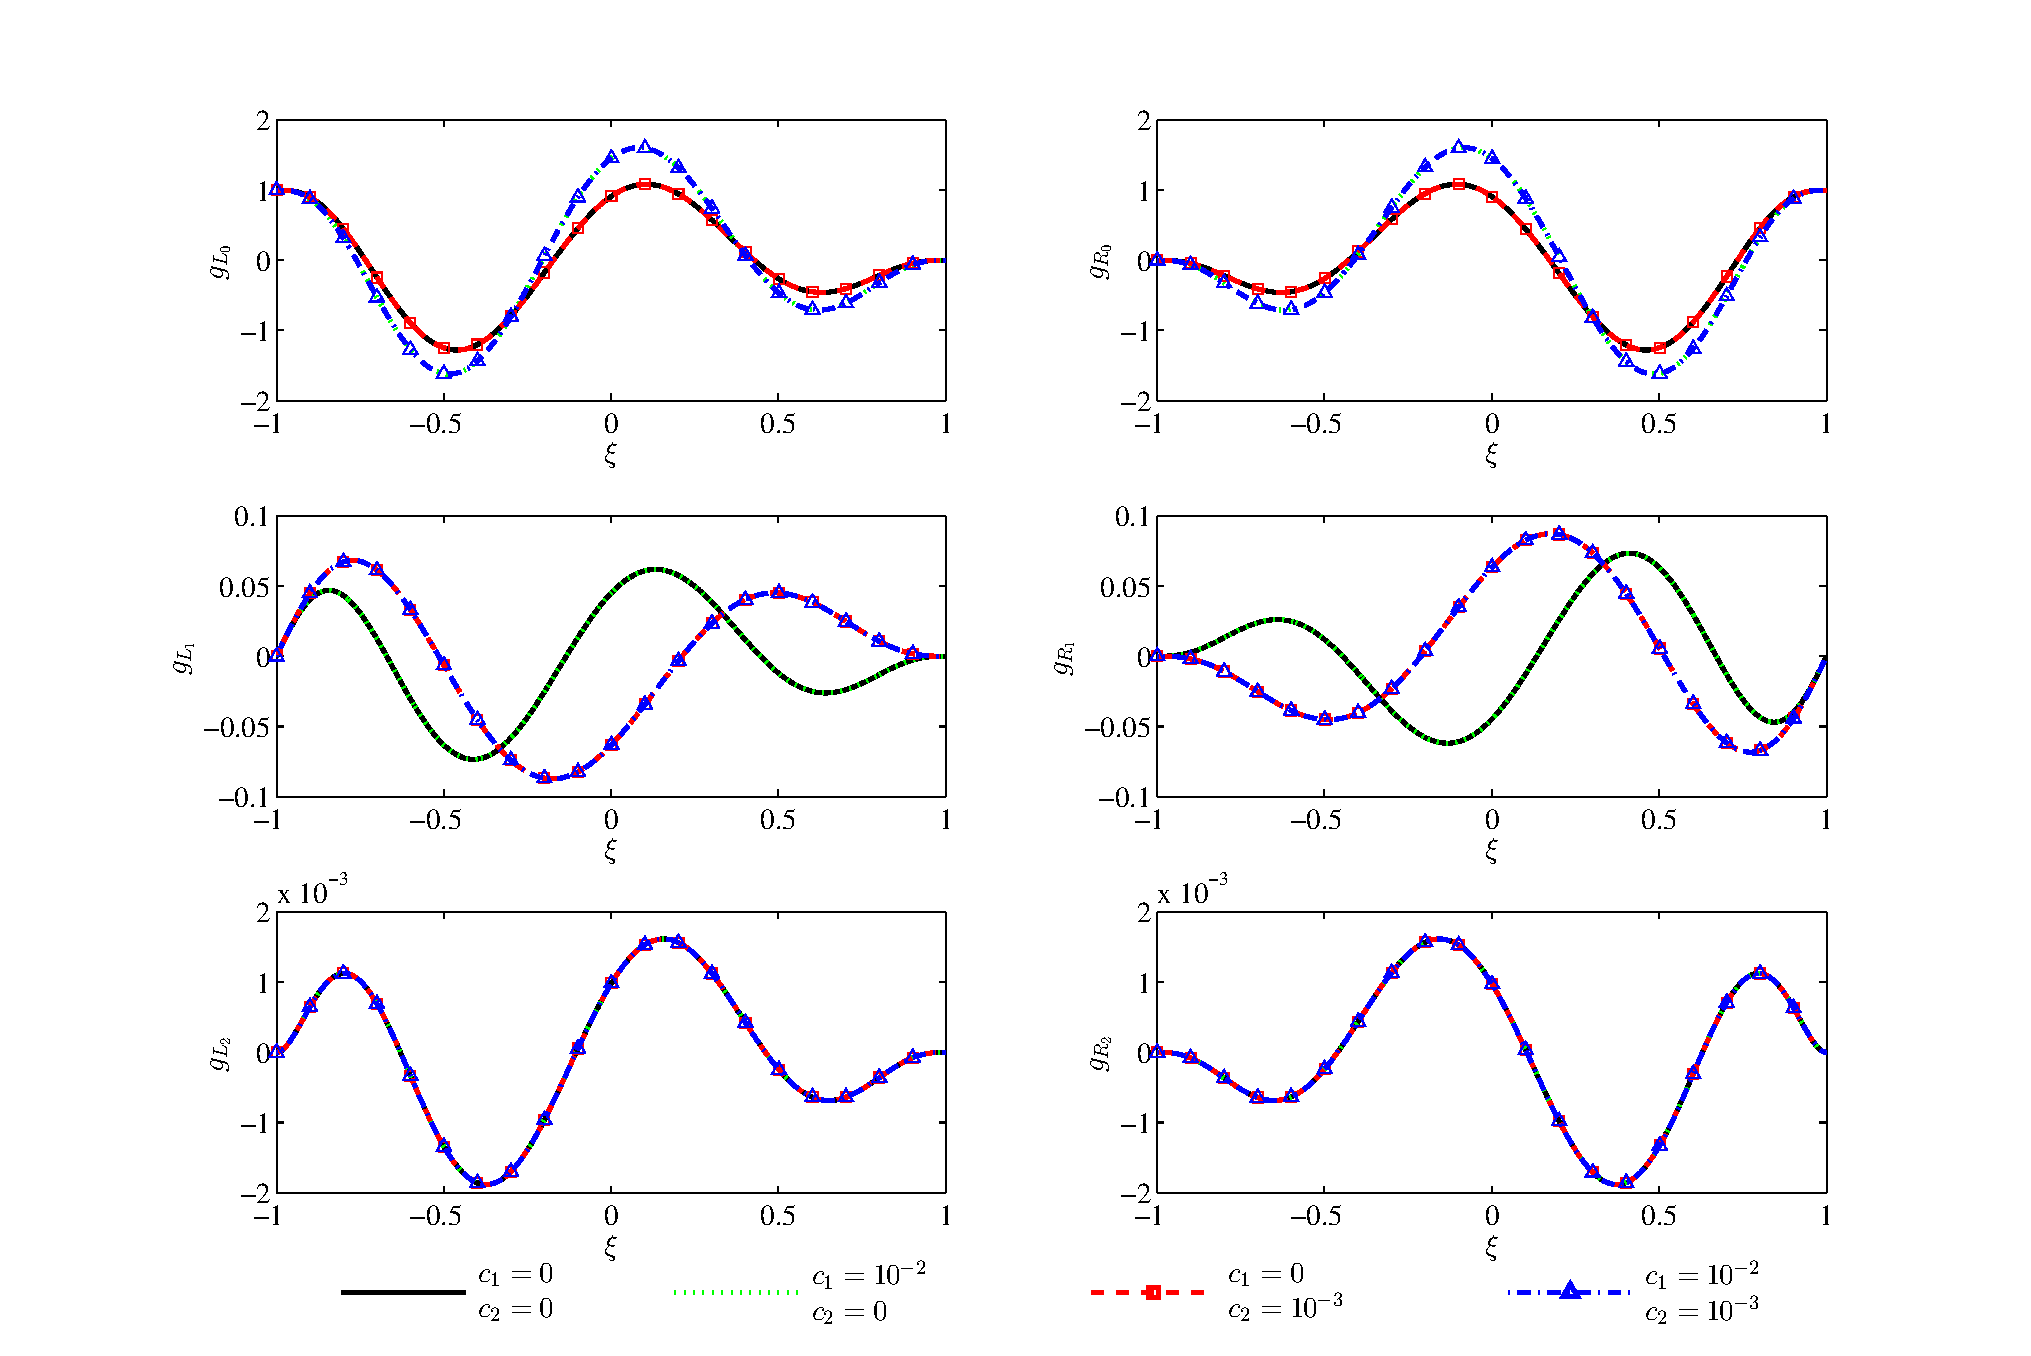
\includegraphics[width =1\textwidth,trim=\Ltrim cm 0cm \Rtrim cm 0cm]{\cmfrdir/Figures/Correction_funcs/C2FR} \caption{Left and right correction functions for the C2FR scheme with $P=3$, in which the zeroth, first, and second derivatives of the corrected flux are continuous} \label{fig:c2_corfunc} 
\end{figure}







\section{Numerical test cases}
\label{sec:num_cases}
In this section we present solutions to the linear advection equation using the C1FR scheme to show that it is stable and achieves the theoretical order of convergence of $P+1$ when the solution is discretized with an order $P$ polynomial. In addition, we present solutions to the linear advection-diffusion equation to demonstrate the ability to change the scheme's dispersion and dissipation properties while maintaining stability.

As can be seen from the derivation of the \gls{c1fr} scheme, the interface flux constants $\alpha_0$ and $\alpha_1$, the norm constants $c_0$ and $c_1$, and the location of the solution points at each element are variable. In this exposition, we will not modify the location of the solution points and use the standard zeroes of the Legendre polynomials. We note that the values of $c_1$ have a direct impact on the scheme's dispersion and dissipation, while --as expected-- the $\alpha_r$ values affect the dissipation only. A future rigorous Fourier analysis would reveal wiser choices for the $c_1$ parameter.


\subsection{Order of Accuracy of C1FR}
\subsubsection{Setup}

The 1-D experiments follow the procedure suggested by Vincent et al.~\cite{vincent2011insights} to estimate  a scheme's order of accuracy isolating interpolation errors. We solve the linear advection equation with advection speed of $a = 1$. The domain was $\Omega = [-10, 10]$ and was discretized in $n = 10, 15, 24, 38, 60$ equispaced elements of orders $P = 1,2,3$. The initial condition was a sine wave with wavenumber $k = 2\pi/20 \approx 0.63$. The advection speed was $1$ and fully upwinded fluxes $\alpha_0 = 0, \alpha_1 = 0$ in Eqn. \eqref{eq:ifluxdef}) were used. The boundary conditions were periodic. The simulation advanced using a fourth order \gls{rk} scheme with a time-step of order $10^{-3}$.

The initial condition was advected for a full domain length, using either standard nodal DG or \gls{c1fr}, and the resulting solution was taken as the reference solution $u_{ref}$. The wave was advected for a further full domain length to obtain the final solution $u_{final}$. The error was calculated by taking the L-2 norm of $u_{ref} - u_{final}$.

\subsubsection{Results and discussion}
Figures \ref{fig:adv_P1},\ref{fig:adv_P2}, and \ref{fig:adv_P3} show the rate of convergence of the solution and its derivative obtained by discretizing the solution wih polynomials of order $P = 1,2,3$, respectively. The slopes of the best fit lines are presented in each figure's caption.

\begin{figure}[h]
\centering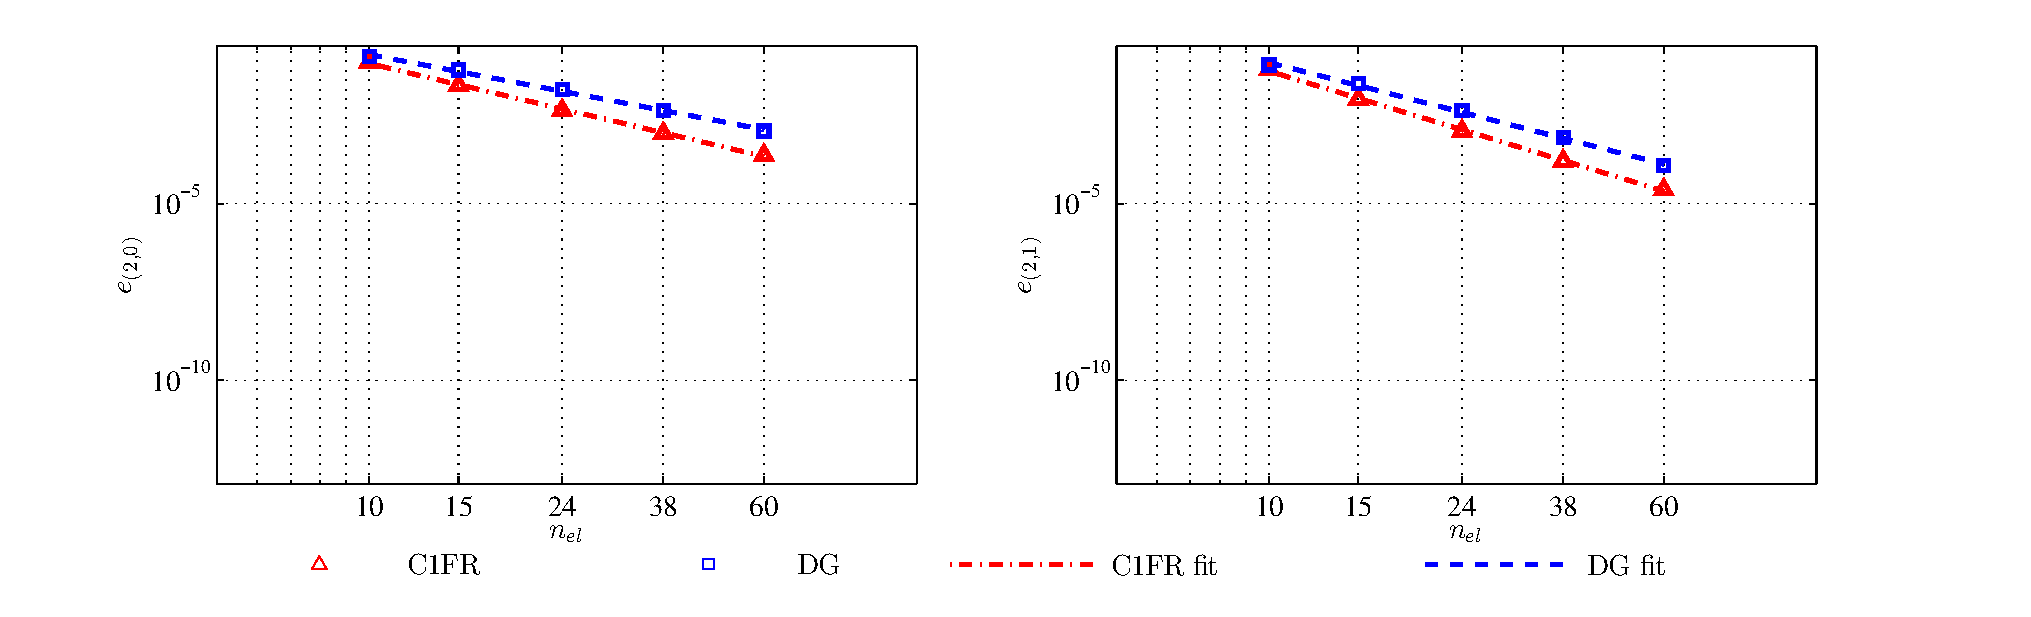
\includegraphics[width=1\textwidth,trim=\Ltrim cm 0cm \Rtrim cm 0cm]{\cmfrdir/Figures/Order_accuracy/P_1}
\caption{L-2 norm of error of advected sine wave and its derivative, $e_{(2,0)}$ and $e_{(2,1)}$ respectively, versus number of elements, for linear advection with polynomial discretization of order $P = 1$. Order of accuracy in solution: \gls{dg}: $2.728$, \gls{c1fr}: $3.374$. Order of accuracy in first derivative: \gls{dg}: $2.691$, \gls{c1fr}: $3.359$.}
\label{fig:adv_P1}
\end{figure}

\begin{figure}[h]
\centering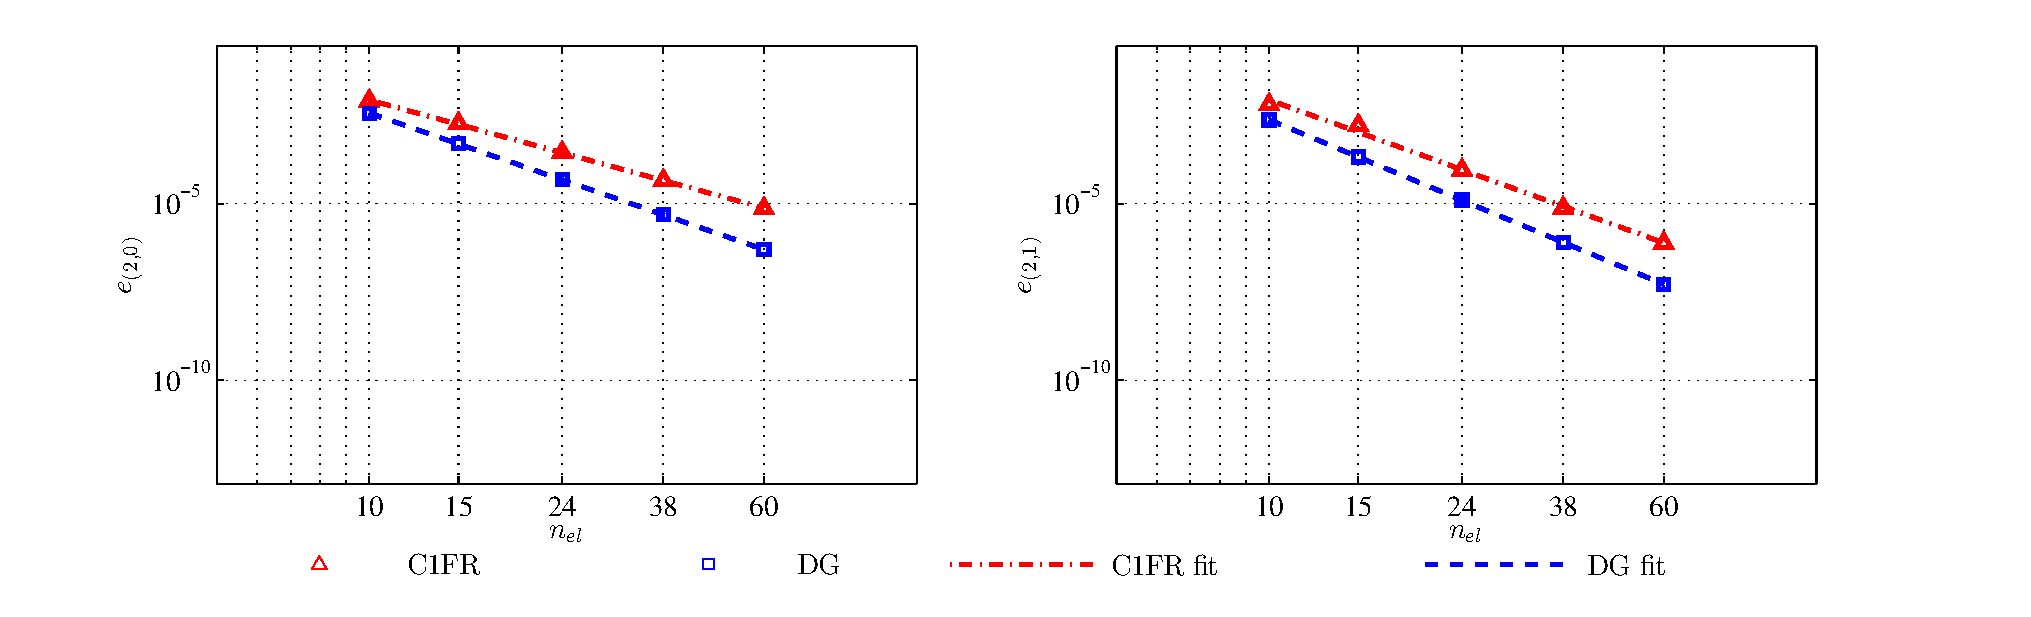
\includegraphics[width=1\textwidth,trim=\Ltrim cm 0cm \Rtrim cm 0cm]{\cmfrdir/Figures/Order_accuracy/P_2}
\caption{L-2 norm of error of advected sine wave and its derivative, $e_{(2,0)}$ and $e_{(2,1)}$ respectively, versus number of elements, for linear advection with polynomial discretization of order $P = 2$. Order of accuracy in solution: \gls{dg}: $4.960$, \gls{c1fr}:  $3.917$ . Order of accuracy in first derivative: \gls{dg}: $4.971$, \gls{c1fr}: $4.178$.}
\label{fig:adv_P2}
\end{figure}

\begin{figure}[h]
\centering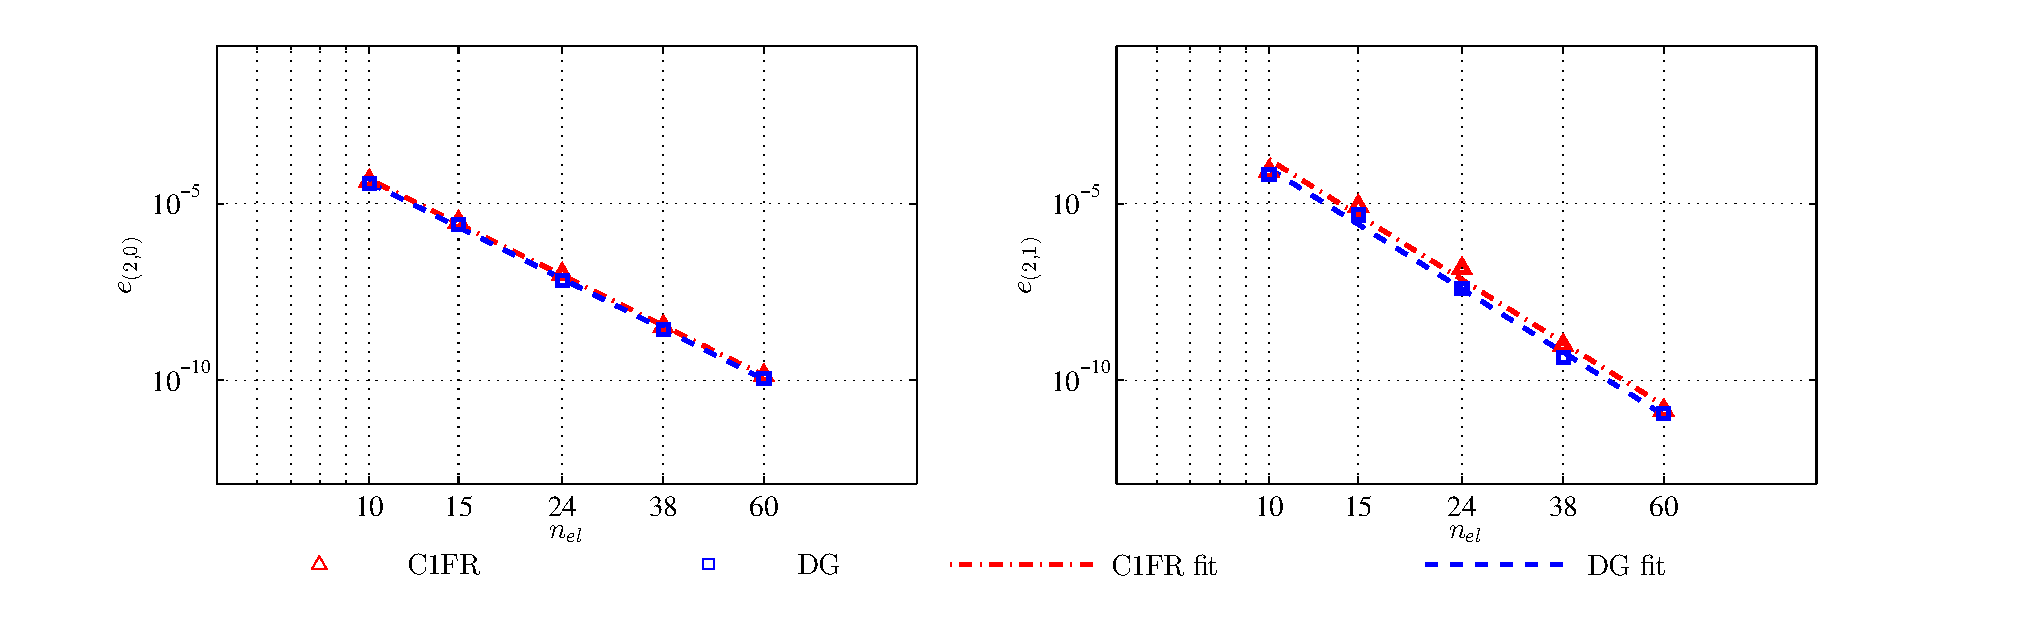
\includegraphics[width=1\textwidth,trim=\Ltrim cm 0cm \Rtrim cm 0cm]{\cmfrdir/Figures/Order_accuracy/P_3}
\caption{L-2 norm of error of advected sine wave and its derivative, $e_{(2,0)}$ and $e_{(2,1)}$ respectively, versus number of elements, for linear advection with polynomial discretization of order $P = 3$. Order of accuracy in solution: \gls{dg}: 7.119, \gls{c1fr}: 7.187. Order of accuracy in first derivative: \gls{dg}: 7.908, \gls{c1fr}: 7.882.}
\label{fig:adv_P3}
\end{figure}

The fact that we recover the expected nodal \gls{dg}'s $2P+1$ order of convergence found by Vincent et al. \cite{vincent2011insights} for $P = 1,2,3$ validates the experimental setup. It is interesting to note that \gls{c1fr} retains \gls{fr}'s even-odd order of convergence behavior: when $P$ is odd, the order of convergence is $2P+1$; while when $P$ is even, the order of convergence is $2P$.

This numerical experiment does not replace a von Neumann analysis, but does show that the scheme is stable, consistent, and maintains the desired order of accuracy. Although we would not expect the scheme to maintain super-convergence properties in real applications --as the interpolation errors are themselves of order $P+1$--, this experiment relieves worries about C1FR's introducing lower order errors.

\subsection{Advection-Diffusion Energy Preservation}
\label{sec:advDiff}
Motivated by the fact that in turbulent simulations the preservation of energy at different scales (or wavenumbers) is of paramount importance, we wanted to explore the potential benefit of having sets of families of stable numerical schemes with modifiable dispersion and dissipation properties.

By solving the linear advection-diffustion equation we are able to assess how much dissipation in different scales is due to numerics as opposed to the nature of the equation.

\subsubsection{Setup}

In these numerical experiments we solve the linear advection-diffusion equation using the C1FR and nodal DG schemes following the approach described by Huynh \cite{huynh2009reconstruction}. In essense, we re-write the diffusion-advection equation as a system of two first order \gls{pde}s as follows
\begin{equation}
\begin{split}
\dd{u}{t} + \dd{q}{x} = 0 \\
q - au + \kappa\dd{u}{x} = 0
\end{split}
\end{equation}

where $a$ is the advection speed, $\kappa$ is the diffusion coefficient, and $q$ is a dummy variable. The desired scheme is used to discretize the spatial differentiation.

In this section, we let $a = 1$, $\kappa = 10^{-2}$. The domain was $\Omega = [-10,10]$ and was discretized in $n = 20$ equispaced elements of polynomial order $P = 5$. The boundary conditions were periodic. The initial conditions were sine waves with low, medium, and high wavenumbers. The wavenumbers were chosen relative to the Nyquist limit of the discretization: 
\[k = \rho (P+1)\pi/h\]
 where $\rho$ is a non-dimensional constant, $P+1$ is the number of solution points in each element of polynomial degree $P$, and $h$ is the size of the element. Note that when $\rho = 1$, the Nyquist limit is reached exactly if the solution points are spaced evenly.

In our experiments, for the low wavenumber $\rho = 0.25$; medium wavenumber $\rho = 0.5$; high wavenumber $\rho = 0.75$. The fluxes were all fully upwinded and in the \gls{c1fr} scheme, $c_1 = -5\cdot10^{-3}$. The solution is advanced with a standard \gls{rk}4 time-stepping scheme. A \gls{cfl} of $0.3$ is used for both schemes. At each timestep, we calculate the square of the L-2 norm of the solution and its derivative, and compare it to the exact corresponding values. $||u||_{(2,m)} $ is the L-2 norm of the $m^{\text{th}}$ derivative of solution $u$.


\subsubsection{Results and discussion}
Fig. \ref{fig:low_wavenumber} shows that both schemes preserve the exact solution and derivative norms of the low wavenumber. On the other hand, \ref{fig:high_wavenumber} shows that both schemes suffer from aliasing and deviate significantly from the exact L-2 norms when the initial solution is a high wavenumber. \gls{c1fr} is somewhat closer to the exact values than nodal \gls{dg} both before and after the norms of the numerical solutions intersect the exact solution's L-2 norm.

Fig. \ref{fig:medium_wavenumber} presents a promising result. \gls{c1fr} preserves the correct L-2 norms of the solution while nodal \gls{dg}'s numerical dissipation affects the energy content of the wave. The L-2 norm of C1FR's solution derivative oscillates around the exact value, while nodal \gls{dg}'s oscillates with similar magnitude trending further below the exact values.


\begin{figure}[h]
\centering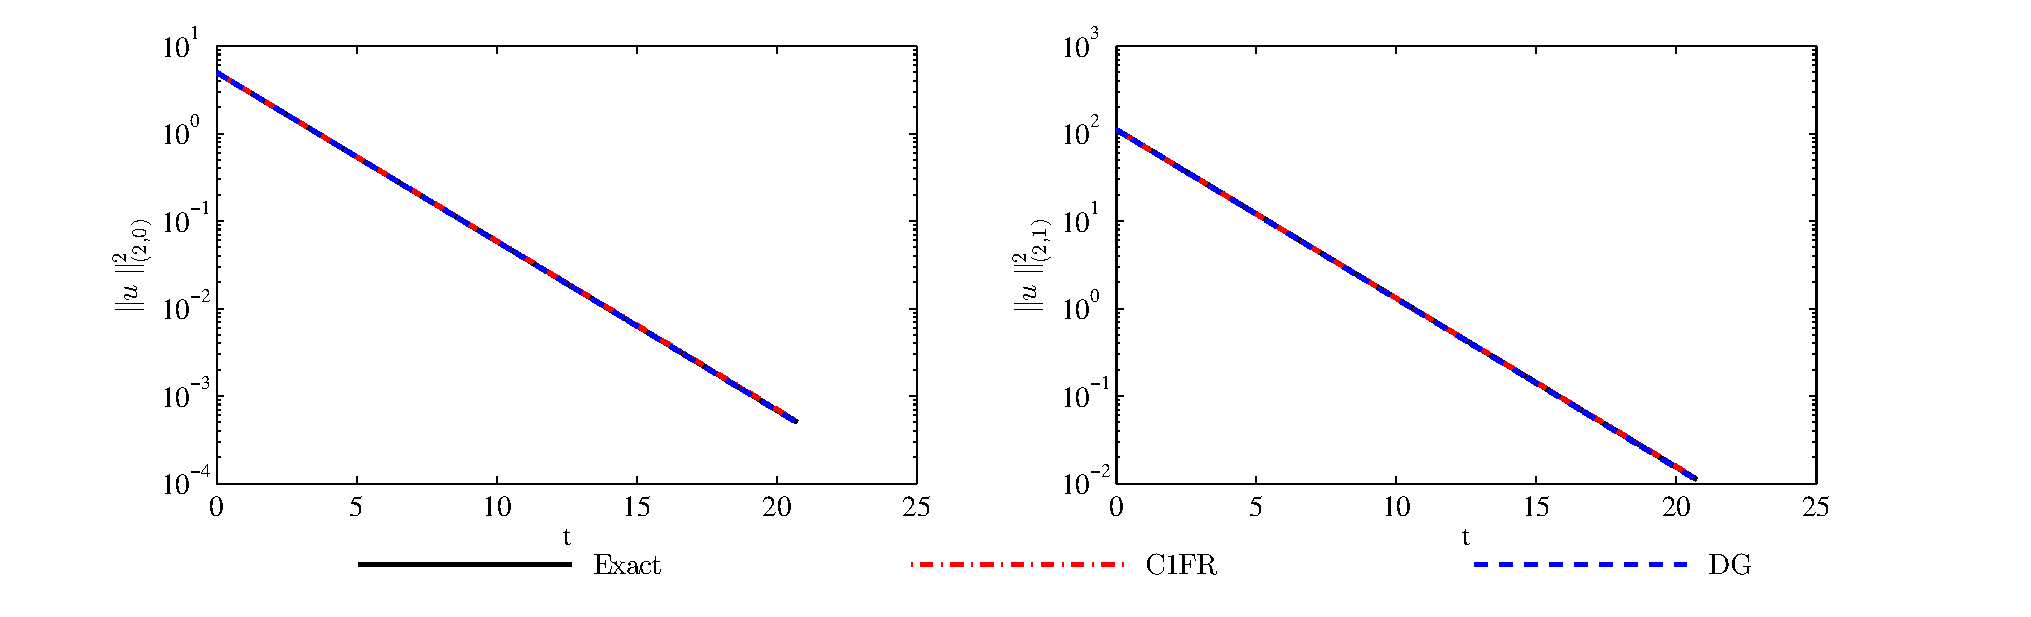
\includegraphics[width=1\textwidth,trim=\Ltrim cm 0cm \Rtrim cm 0cm]{\cmfrdir/Figures/Test_adv_diff/low_k}
\caption{Time history of norms of numerical solutions to the advection-diffusion equation and their first derivative. Initial condition is a sine wave with low wavenumber: $k = 0.25 (P+1)\pi/h$, $P = 3$, $h = 1$.}
\label{fig:low_wavenumber}
\end{figure}

\begin{figure}[h]
\centering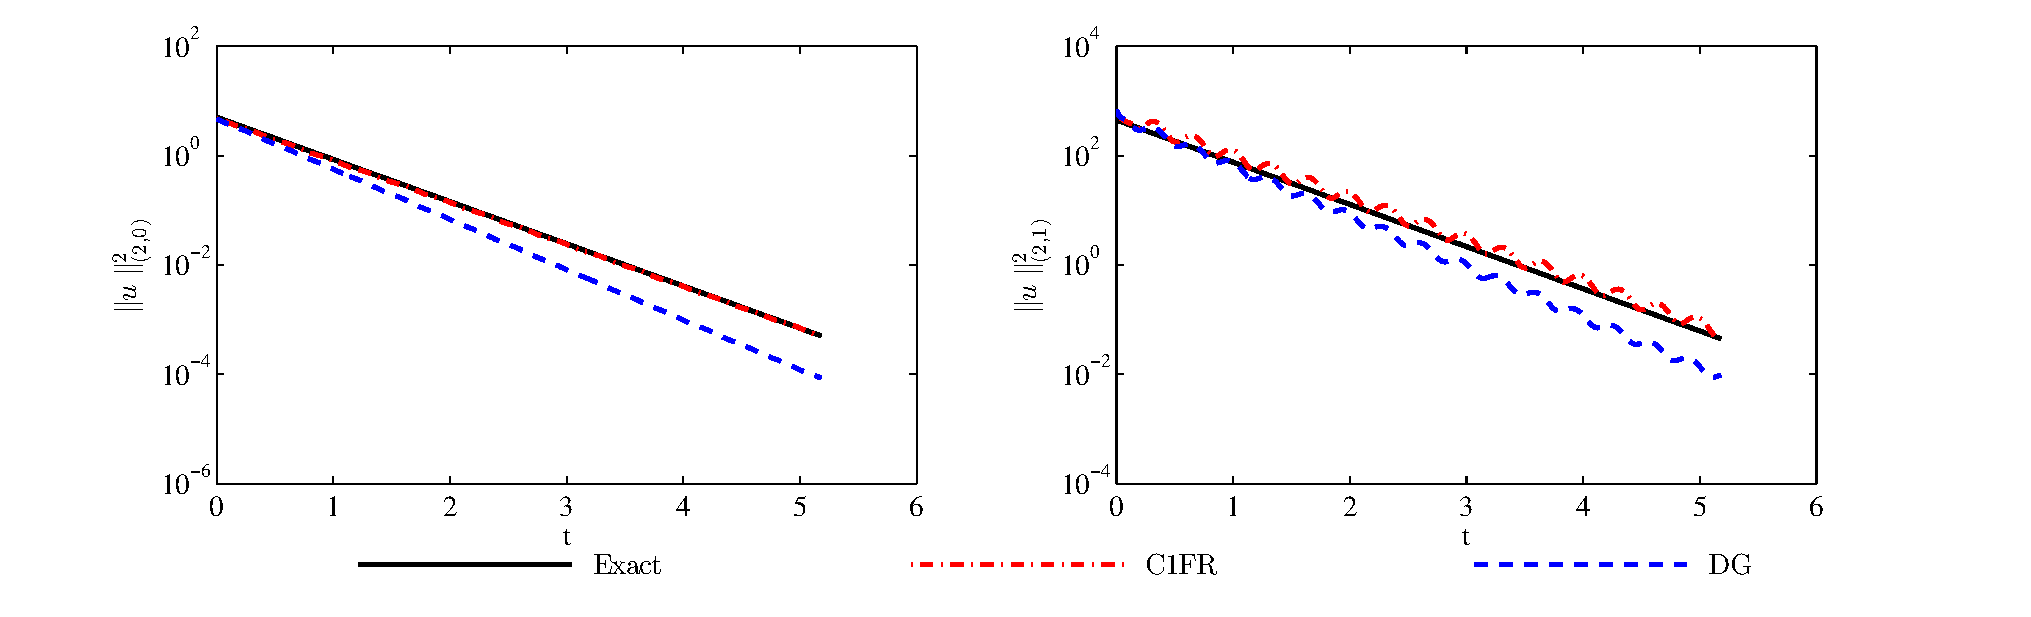
\includegraphics[width=1\textwidth,trim=\Ltrim cm 0cm \Rtrim cm 0cm]{\cmfrdir/Figures/Test_adv_diff/med_k}
\caption{Time history of norms of numerical solutions to the advection-diffusion equation and their first derivative. Initial condition is a sine wave with medium wavenumber: $k = 0.5 (P+1)\pi/h$, $P = 3$, $h = 1$.}
\label{fig:medium_wavenumber}
\end{figure}

\begin{figure}[h]
\centering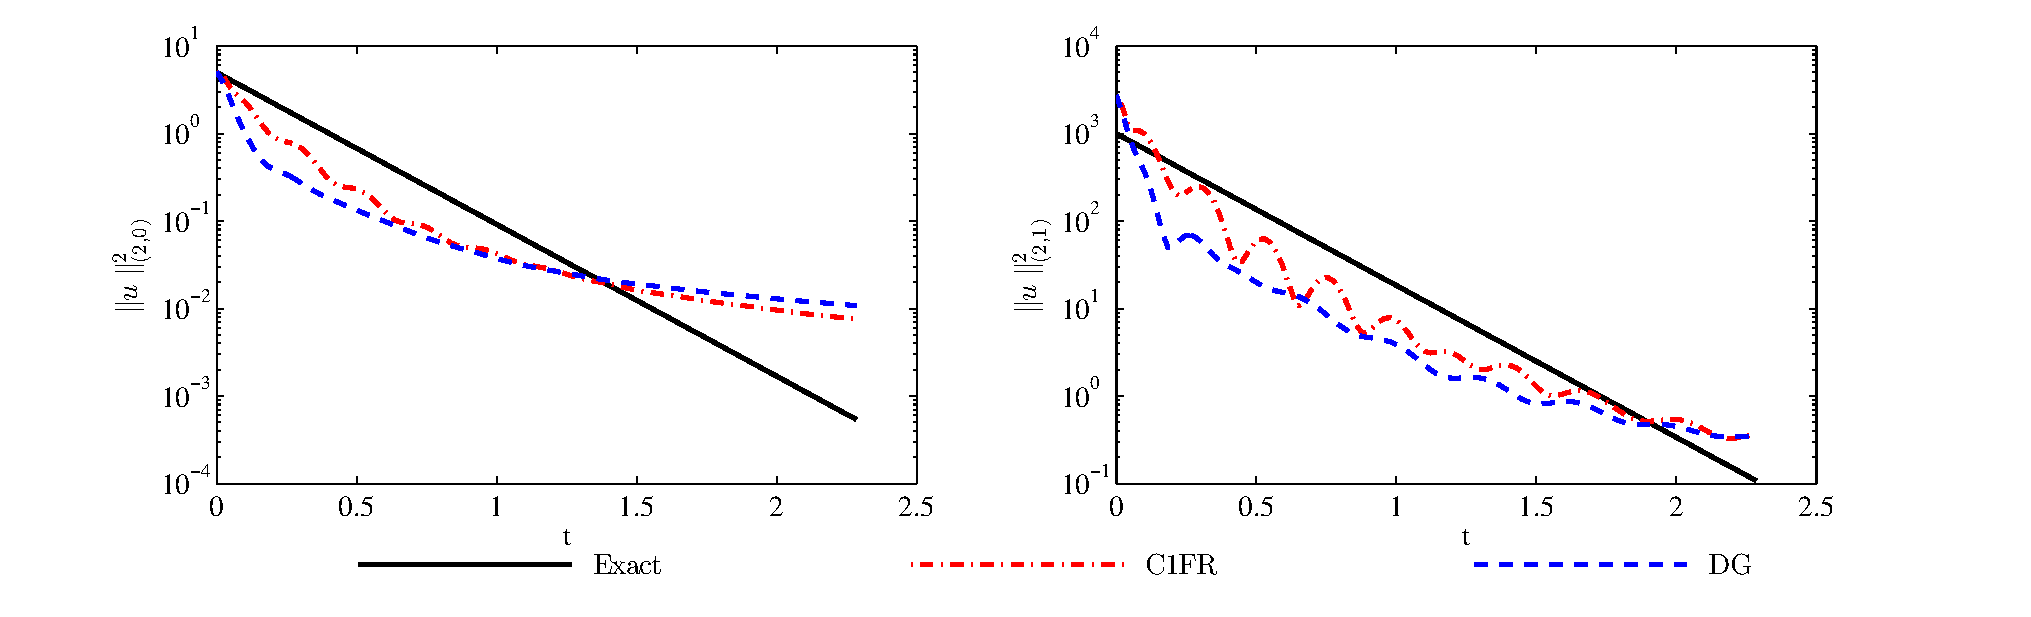
\includegraphics[width=1\textwidth,trim=\Ltrim cm 0cm \Rtrim cm 0cm]{\cmfrdir/Figures/Test_adv_diff/high_k}
\caption{Time history of norms of numerical solutions to the advection-diffusion equation and their first derivative. Initial condition is a sine wave with high wavenumber: $k = 0.75 (P+1)\pi/h$, $P = 3$, $h = 1$.}
\label{fig:high_wavenumber}
\end{figure}

%_ %_ %_ %_ %_ %_ %_ %_ %_ %_ %_ %_ %_ %_ %_ %_ %_ %
%\begin{figure}[h]
%\centering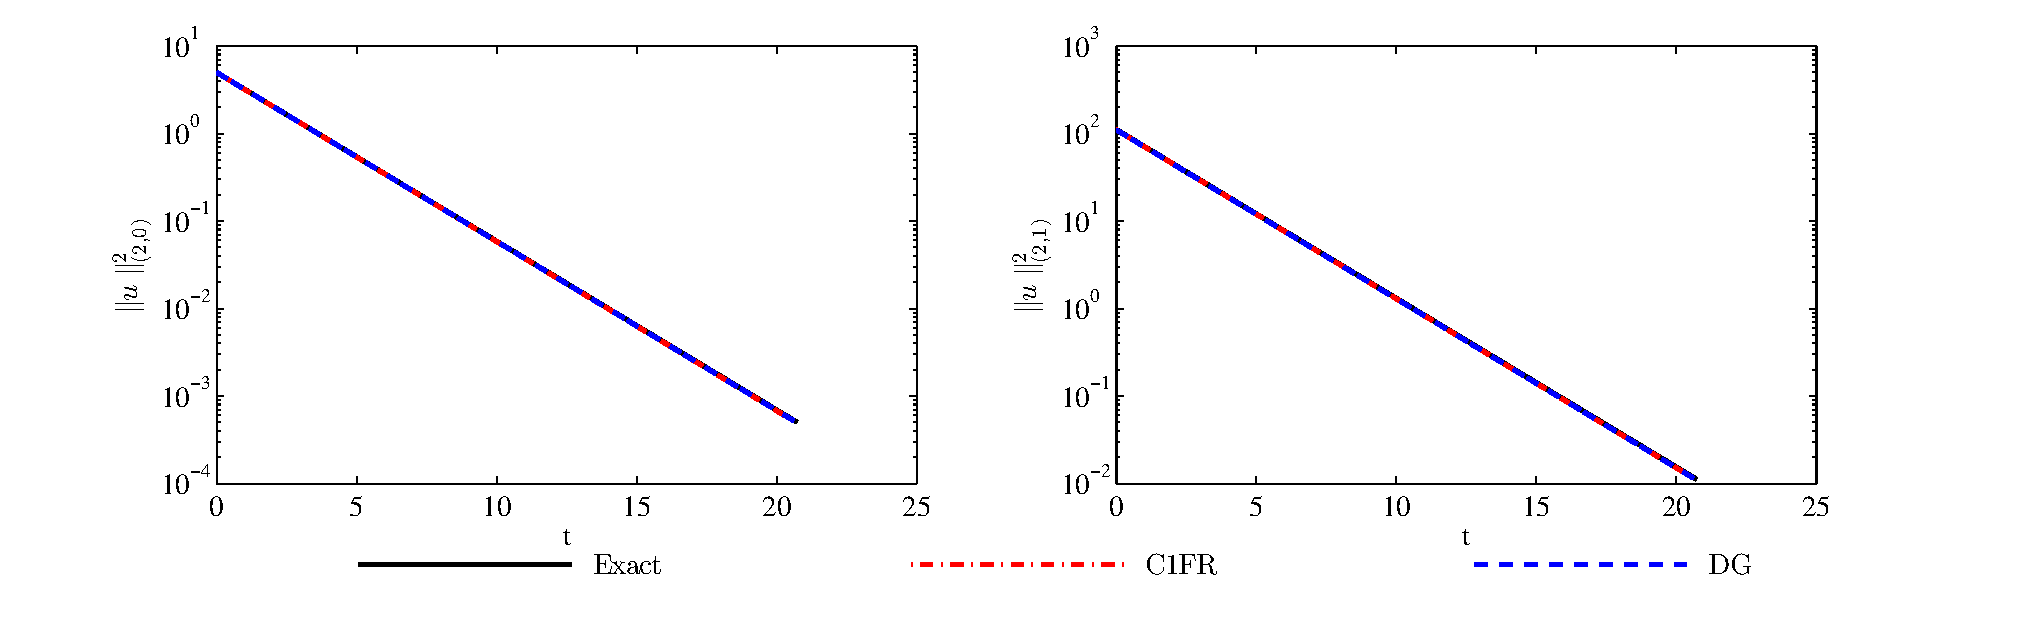
\includegraphics[width=1\textwidth,trim=\Ltrim cm 0cm \Rtrim cm 0cm]{Figures/Test_adv_diff/low_k_c_5e-3}
%\caption{Time history of norms of numerical solutions to the advection-diffusion equation and their first derivative. Initial condition is a sine wave with low wavenumber: $k = 0.25 (P+1)\pi/h$, $P = 3$, $h = 1$.}
%\label{fig:low_wavenumber2}
%\end{figure}
%
%\begin{figure}[h]
%\centering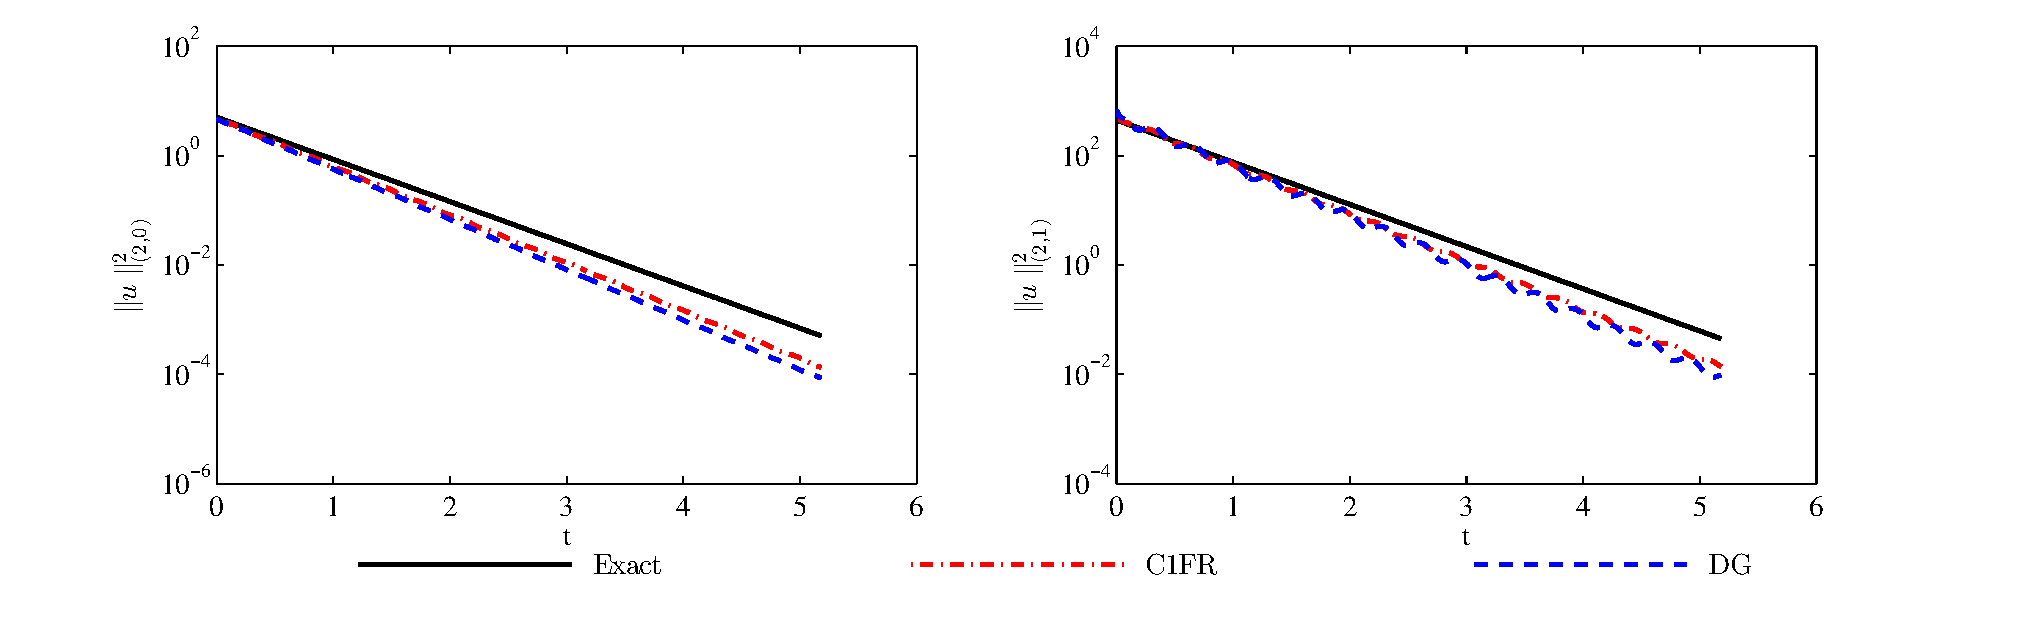
\includegraphics[width=1\textwidth,trim=\Ltrim cm 0cm \Rtrim cm 0cm]{Figures/Test_adv_diff/med_k_c_5e-3}
%\caption{Time history of norms of numerical solutions to the advection-diffusion equation and their first derivative. Initial condition is a sine wave with medium wavenumber: $k = 0.5 (P+1)\pi/h$, $P = 3$, $h = 1$.}
%\label{fig:medium_wavenumber2}
%\end{figure}
%
%\begin{figure}[h]
%\centering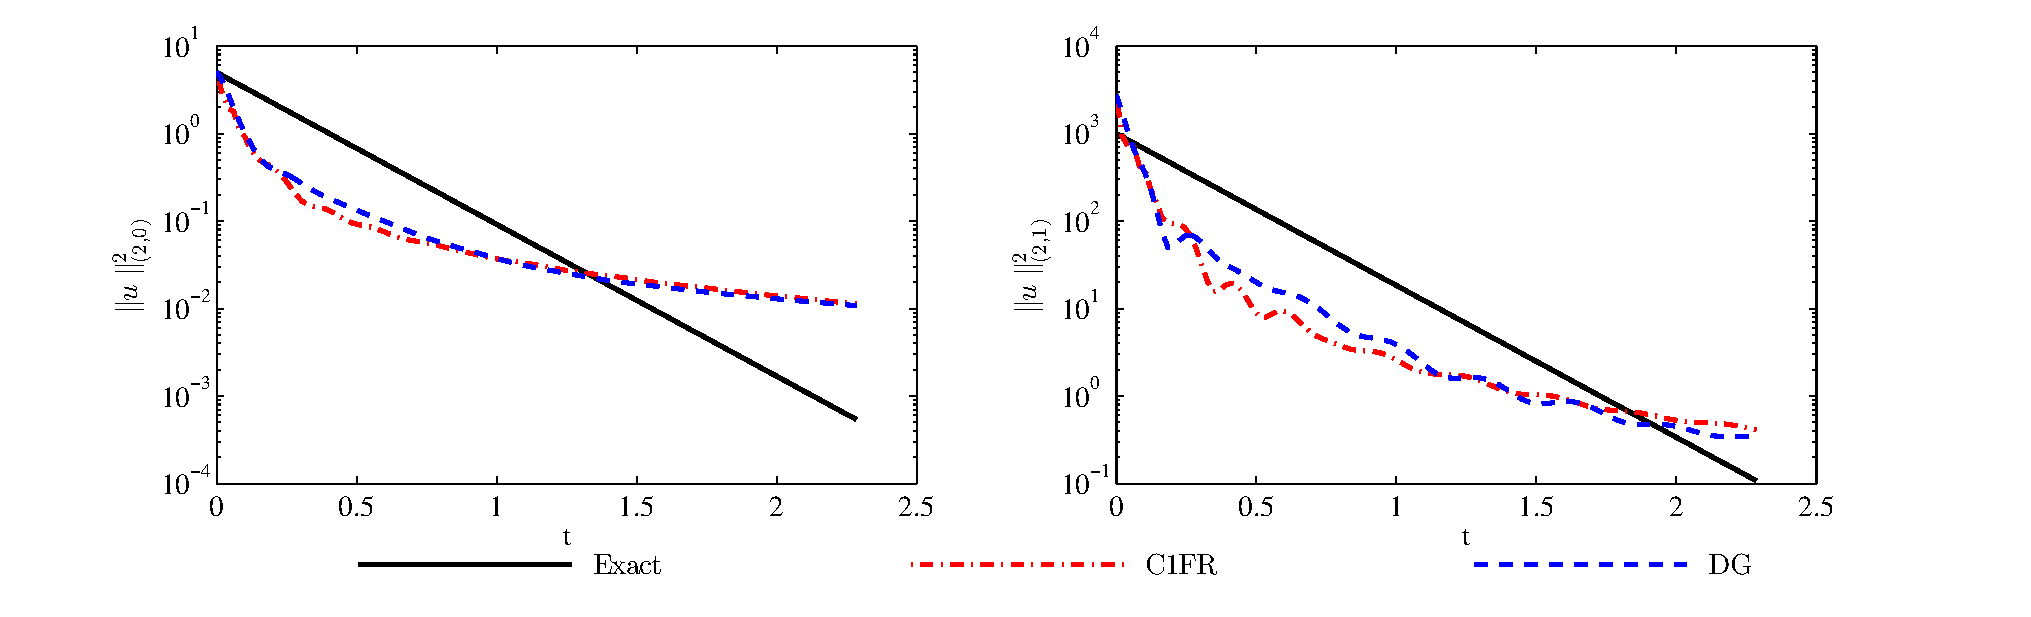
\includegraphics[width=1\textwidth,trim=\Ltrim cm 0cm \Rtrim cm 0cm]{Figures/Test_adv_diff/high_k_c_5e-3}
%\caption{Time history of norms of numerical solutions to the advection-diffusion equation and their first derivative. Initial condition is a sine wave with high wavenumber: $k = 0.75 (P+1)\pi/h$, $P = 3$, $h = 1$.}
%\label{fig:high_wavenumber2}
%\end{figure}

%_ %_ %_ %_ %_ %_ %_ %_ %_ %_ %_ %_ %_ %_ %_ %_ %_ %

%\begin{figure}
%\centering
%\subfigure[fig a]{\label{fig:high_wavenumber} 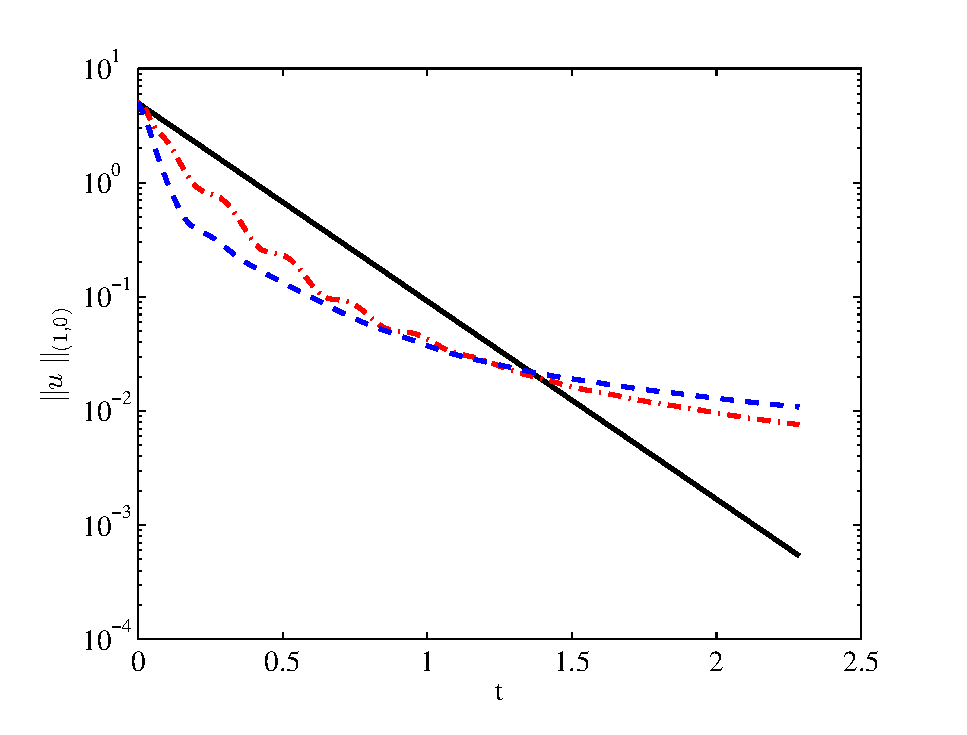
\includegraphics[width = .5\textwidth]{Figures/Test_adv_diff/eN0_high_k}
%\caption{energy history}}

%\end{subfig}
%\end{figure}



\section{Conclusions}

We have presented a natural extension of the \gls{fr} approach. The \gls{cmfr} schemes guarantee 1-D linear stability and introduce an arbitrary number of parameters that modify the scheme's dispersive and dissipative properties. The addition of these parameters require the representation of the reconstructed flux to be $p+1$ or higher, where $p$ is the order of the polynomial used to represent the conservative solution.

 We have shown the derivation of the \gls{c1fr} scheme, which has reconstructed fluxes continuous in the zeroth and first derivatives accross elements. This scheme, with a particular selection of its free parameter, was able to preserve the energy of an advected and diffused wave with a medium wavenumber better than the nodal \gls{dg} scheme. Certainly, this one example cannot be said to be generalizable. Nevertheless, it calls for a Von Neumann analysis to assess the impact of the free parameter on the scheme's properties. As the general \gls{cmfr} schemes have arbitrarily many such parameters, this analysis should be generalizable.

A major complication with the general \gls{cmfr} schemes is that the correction functions do depend on the element's Jacobian, so they are not as general and element-agnostic as those in the original \gls{fr} schemes. However, as shown by Allaneau~\cite{allaneau2011connections}, it is possible to formulate some \gls{fr} schemes as filtered \gls{dg} schemes without the need to find the correction functions explicitly. A similar analysis with the \gls{fr} schemes could yield element-dependent filtered \gls{dg} schemes whose properties can be understood or optimized in the \gls{cmfr} framework.

Future work should include numerical experiments in 2-D and 3-D using tensor product elements to assess the extent to which the stability guarantees in 1-D translate to other dimensions. In addition, it is still unclear if the degree of continuity of the corrected fluxes could be beneficial in the solution of high order partial differential equations.

\newpage
\section*{References}
\bibliographystyle{elsarticle-num}
\bibliography{references2}


\end{document}
